
\documentclass[10pt]{beamer}
\usetheme{metropolis}

% ── Packages ──
\usepackage{amsmath,amssymb,amsthm}
\usepackage{tikz}
\usetikzlibrary{positioning,arrows.meta,fit,matrix,backgrounds,calc,shapes.geometric}
\usepackage{graphicx}
\usepackage{array}
\usepackage{etoolbox}

% ── Theorem environments ──
\theoremstyle{definition}
\newtheorem{defi}{Definition}[section]
\newtheorem{prop}{Proposition}[section]
\newtheorem{thm}{Theorem}[section]
\newtheorem{cor}{Corollary}[section]

% Custom theorem styles with colors
\setbeamercolor{block title}{bg=red!75!black,fg=white}
\setbeamercolor{block body}{bg=yellow!10!white}

\AtBeginEnvironment{prop}{%
  \setbeamercolor{block title}{bg=yellow!75!black,fg=black}%
  \setbeamercolor{block body}{bg=yellow!10!white}%
}
\AtEndEnvironment{prop}{%
  \setbeamercolor{block title}{bg=red!75!black,fg=white}%
}

\AtBeginEnvironment{thm}{%
  \setbeamercolor{block title}{bg=yellow!75!black,fg=black}%
  \setbeamercolor{block body}{bg=yellow!10!white}%
}
\AtEndEnvironment{thm}{%
  \setbeamercolor{block title}{bg=red!75!black,fg=white}%
}

\AtBeginEnvironment{cor}{%
  \setbeamercolor{block title}{bg=yellow!75!black,fg=black}%
  \setbeamercolor{block body}{bg=yellow!10!white}%
}
\AtEndEnvironment{cor}{%
  \setbeamercolor{block title}{bg=red!75!black,fg=white}%
}

% ── Highlighting ──
\newcommand{\x}[1]{\alert{\textbf{#1}}}

% ── Color shortcuts ──
\newcommand{\rd}[1]{{\color{red!70!black}#1}}
\newcommand{\bl}[1]{{\color{blue!70!black}#1}}
\newcommand{\gn}[1]{{\color{green!60!black}#1}}

\title{Lecture 12: Determinant}
\subtitle{MATH203 Applied Linear Algebra}
\date{}
\titlegraphic{}

\begin{document}
\maketitle


% ═══════════════════════════════════════
% §1 FROM AREA TO DETERMINANT
% ADR: AUDIENCE EMOTION — students need to SEE area before any axioms.
% Start with a concrete geometric puzzle on a grid. The parallelogram
% area question is visceral — "how big is this shape?" needs no
% prerequisites. The three properties (multilinearity, alternating,
% normalization) are DISCOVERED from geometric intuition, not stated
% as axioms. The ad-bc formula is derived via rectangle cut-out,
% giving students a visual proof they can reconstruct from memory.
% ═══════════════════════════════════════
\section{From Area to Determinant}

% ── Frame 1: Tension opening ──────────────────────────────
% ADR: Start with a question, not a definition.
\begin{frame}{How Big Is This Shape?}

Suppose each small square on the grid has area $1$.

\begin{center}
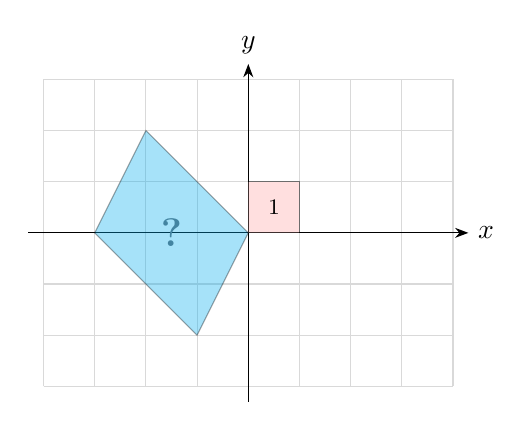
\begin{tikzpicture}[scale=0.65]
  % Grid
  \draw[gray!30, step=1] (-4,-3) grid (4,3);
  \draw[-{Stealth}] (-4.3,0) -- (4.3,0) node[right]{$x$};
  \draw[-{Stealth}] (0,-3.3) -- (0,3.3) node[above]{$y$};

  % Unit square
  \filldraw[fill=pink, opacity=0.5] (0,0) -- (1,0) -- (1,1) -- (0,1) -- cycle;
  \node at (0.5, 0.5) {\footnotesize $1$};

  % Parallelogram: v1=(-1,-2), v2=(-2,2)
  \filldraw[fill=cyan, opacity=0.35] (0,0) -- (-1,-2) -- (-3,0) -- (-2,2) -- cycle;
  \node[font=\Large, cyan!60!black] at (-1.5, 0) {\textbf{?}};
\end{tikzpicture}
\end{center}

\vfill
How do you calculate the {\color{cyan!60!black}\textbf{blue area}}?

\end{frame}


% ── Frame 2: Area depends on two vectors ──────────────────
% ADR: Connect the shape to its two side vectors. Introduce det as notation.
\begin{frame}{Two Vectors Determine the Shape}

The blue shape is a \x{parallelogram} — determined by two side vectors:

\begin{center}
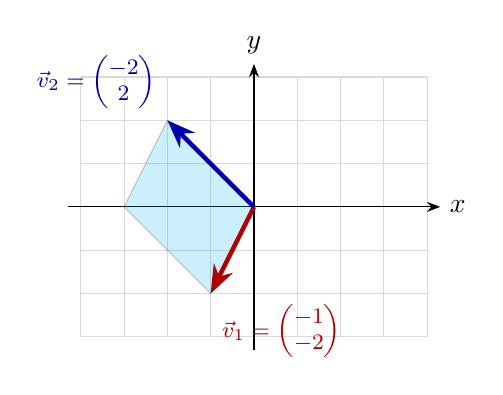
\begin{tikzpicture}[scale=0.55]
  \draw[gray!30, step=1] (-4,-3) grid (4,3);
  \draw[-{Stealth}] (-4.3,0) -- (4.3,0) node[right]{$x$};
  \draw[-{Stealth}] (0,-3.3) -- (0,3.3) node[above]{$y$};

  \filldraw[fill=cyan, opacity=0.2] (0,0) -- (-1,-2) -- (-3,0) -- (-2,2) -- cycle;

  \draw[-{Stealth}, ultra thick, red!70!black] (0,0) -- (-1,-2)
    node[below right]{\footnotesize $\vec{v}_1 = \begin{pmatrix} -1 \\ -2 \end{pmatrix}$};
  \draw[-{Stealth}, ultra thick, blue!70!black] (0,0) -- (-2,2)
    node[above left]{\footnotesize $\vec{v}_2 = \begin{pmatrix} -2 \\ 2 \end{pmatrix}$};
\end{tikzpicture}
\end{center}

We write: \quad $\det\begin{pmatrix} -1 & -2 \\ -2 & 2 \end{pmatrix} = $ {\color{cyan!60!black}\textbf{signed blue area}}

\vfill
``$\det$'' eats two column vectors and returns the \x{signed area} of their parallelogram.

\end{frame}


% ── Frame 3: Easy case — axis-aligned ─────────────────────
% ADR: Build from the simplest possible case.
\begin{frame}{The Easy Case: Axis-Aligned Rectangle}

When both vectors point along the axes, the parallelogram is a \x{rectangle}:

\begin{center}
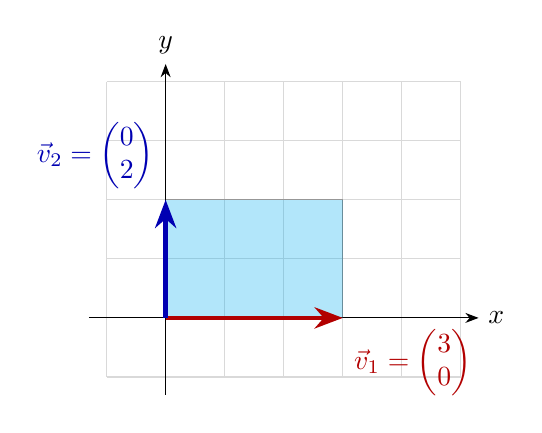
\begin{tikzpicture}[scale=0.75]
  \draw[gray!30, step=1] (-1,-1) grid (5,4);
  \draw[-{Stealth}] (-1.3,0) -- (5.3,0) node[right]{$x$};
  \draw[-{Stealth}] (0,-1.3) -- (0,4.3) node[above]{$y$};

  \filldraw[fill=cyan, opacity=0.3] (0,0) -- (3,0) -- (3,2) -- (0,2) -- cycle;

  \draw[-{Stealth}, ultra thick, red!70!black] (0,0) -- (3,0)
    node[below right]{$\vec{v}_1 = \begin{pmatrix} 3 \\ 0 \end{pmatrix}$};
  \draw[-{Stealth}, ultra thick, blue!70!black] (0,0) -- (0,2)
    node[above left]{$\vec{v}_2 = \begin{pmatrix} 0 \\ 2 \end{pmatrix}$};
\end{tikzpicture}
\end{center}

$$
\text{Area} = \text{base} \times \text{height} = 3 \times 2 = \x{6}
$$

\end{frame}


% ── Frame 4: Height points down ───────────────────────────
% ADR: Introduce the concept of signed area through a concrete surprise.
\begin{frame}{What If the Height Points Down?}

Now $\vec{v}_2$ points \x{downward}:

\begin{center}
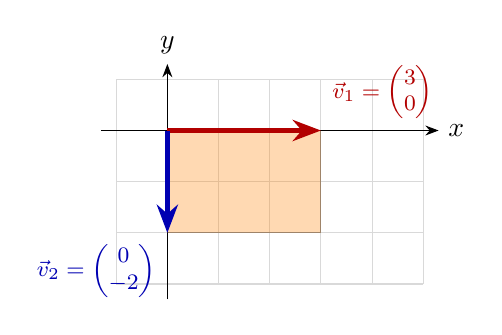
\begin{tikzpicture}[scale=0.65]
  \draw[gray!30, step=1] (-1,-3) grid (5,1);
  \draw[-{Stealth}] (-1.3,0) -- (5.3,0) node[right]{$x$};
  \draw[-{Stealth}] (0,-3.3) -- (0,1.3) node[above]{$y$};

  \filldraw[fill=orange, opacity=0.3] (0,0) -- (3,0) -- (3,-2) -- (0,-2) -- cycle;

  \draw[-{Stealth}, ultra thick, red!70!black] (0,0) -- (3,0)
    node[above right]{\footnotesize $\vec{v}_1 = \begin{pmatrix} 3 \\ 0 \end{pmatrix}$};
  \draw[-{Stealth}, ultra thick, blue!70!black] (0,0) -- (0,-2)
    node[below left]{\footnotesize $\vec{v}_2 = \begin{pmatrix} 0 \\ -2 \end{pmatrix}$};
\end{tikzpicture}
\end{center}

$$
\text{Signed area} = \text{base} \times \text{height} = 3 \times (-2) = \x{-6}
$$

Same size, but the sign tells us the \x{orientation} has changed.

\end{frame}


% ── Frame 5: Oriented area ────────────────────────────────
% ADR: Formalize the sign convention with side-by-side comparison.
\begin{frame}{Oriented Area}

This signed area is called the \x{oriented area}.

\vfill

\begin{columns}[T]
\begin{column}{0.48\textwidth}
\begin{center}
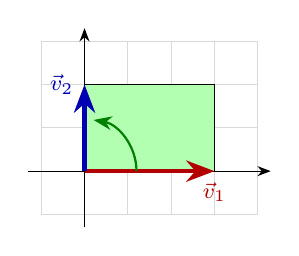
\begin{tikzpicture}[scale=0.55]
  \draw[gray!30, step=1] (-1,-1) grid (4,3);
  \draw[-{Stealth}] (-1.3,0) -- (4.3,0);
  \draw[-{Stealth}] (0,-1.3) -- (0,3.3);
  \filldraw[fill=green!30] (0,0) -- (3,0) -- (3,2) -- (0,2) -- cycle;
  \draw[-{Stealth}, ultra thick, red!70!black] (0,0) -- (3,0) node[below]{\footnotesize $\vec{v}_1$};
  \draw[-{Stealth}, ultra thick, blue!70!black] (0,0) -- (0,2) node[left]{\footnotesize $\vec{v}_2$};

  % CCW arc
  \draw[-{Stealth}, thick, green!50!black] (1.2,0)
    arc[start angle=0, end angle=80, radius=1.2];
\end{tikzpicture}

\vspace{0.2cm}
$\vec{v}_2$ is \x{counterclockwise}

from $\vec{v}_1$: \quad Area $> 0$
\end{center}
\end{column}
\begin{column}{0.48\textwidth}
\begin{center}
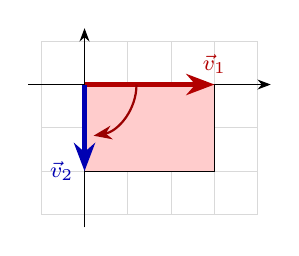
\begin{tikzpicture}[scale=0.55]
  \draw[gray!30, step=1] (-1,-3) grid (4,1);
  \draw[-{Stealth}] (-1.3,0) -- (4.3,0);
  \draw[-{Stealth}] (0,-3.3) -- (0,1.3);
  \filldraw[fill=red!20] (0,0) -- (3,0) -- (3,-2) -- (0,-2) -- cycle;
  \draw[-{Stealth}, ultra thick, red!70!black] (0,0) -- (3,0) node[above]{\footnotesize $\vec{v}_1$};
  \draw[-{Stealth}, ultra thick, blue!70!black] (0,0) -- (0,-2) node[left]{\footnotesize $\vec{v}_2$};

  % CW arc
  \draw[-{Stealth}, thick, red!60!black] (1.2,0)
    arc[start angle=0, end angle=-80, radius=1.2];
\end{tikzpicture}

\vspace{0.2cm}
$\vec{v}_2$ is \x{clockwise}

from $\vec{v}_1$: \quad Area $< 0$
\end{center}
\end{column}
\end{columns}

\end{frame}


% ── Frame 6: Transition — what properties? ────────────────
% ADR: Whitespace transition. Tension question before listing properties.
\begin{frame}{}
\vfill
\begin{center}
{\Large What \x{properties} should ``signed area'' satisfy?}
\end{center}
\vfill
\end{frame}


% ── Frame 7: Additivity ──────────────────────────────────
% ADR: The hardest property to visualize. Show the geometric decomposition:
% fix v2 as base, the big parallelogram splits into two pieces along v1.
\begin{frame}{Property 1: Additivity}

Fix the base $\vec{v}_2$. If we \x{add} the heights, the areas \x{add}:

\begin{center}
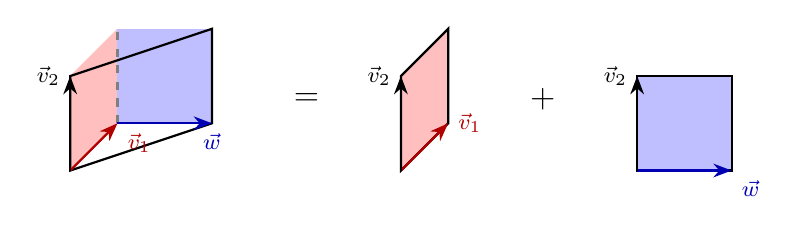
\begin{tikzpicture}[scale=0.6]
  % Left: combined parallelogram v1+w=(3,1), v2=(0,2)
  %   v1=(1,1), w=(2,0)
  %   Split line: (1,1)--(1,3)
  \fill[red!25] (0,0) -- (1,1) -- (1,3) -- (0,2) -- cycle;
  \fill[blue!25] (1,1) -- (3,1) -- (3,3) -- (1,3) -- cycle;
  \draw[thick] (0,0) -- (3,1) -- (3,3) -- (0,2) -- cycle;
  \draw[dashed, thick, gray] (1,1) -- (1,3);

  \draw[-{Stealth}, thick, red!70!black] (0,0) -- (1,1)
    node[below right, font=\footnotesize]{$\vec{v}_1$};
  \draw[-{Stealth}, thick, blue!70!black] (1,1) -- (3,1)
    node[below, font=\footnotesize]{$\vec{w}$};
  \draw[-{Stealth}, thick] (0,0) -- (0,2)
    node[left, font=\footnotesize]{$\vec{v}_2$};

  % "="
  \node[font=\large] at (5, 1.5) {$=$};

  % Middle: red piece alone
  \begin{scope}[shift={(7,0)}]
    \fill[red!25] (0,0) -- (1,1) -- (1,3) -- (0,2) -- cycle;
    \draw[thick] (0,0) -- (1,1) -- (1,3) -- (0,2) -- cycle;
    \draw[-{Stealth}, thick, red!70!black] (0,0) -- (1,1)
      node[right, font=\footnotesize]{$\vec{v}_1$};
    \draw[-{Stealth}, thick] (0,0) -- (0,2)
      node[left, font=\footnotesize]{$\vec{v}_2$};
  \end{scope}

  % "+"
  \node[font=\large] at (10, 1.5) {$+$};

  % Right: blue piece at origin
  \begin{scope}[shift={(12,0)}]
    \fill[blue!25] (0,0) -- (2,0) -- (2,2) -- (0,2) -- cycle;
    \draw[thick] (0,0) -- (2,0) -- (2,2) -- (0,2) -- cycle;
    \draw[-{Stealth}, thick, blue!70!black] (0,0) -- (2,0)
      node[below right, font=\footnotesize]{$\vec{w}$};
    \draw[-{Stealth}, thick] (0,0) -- (0,2)
      node[left, font=\footnotesize]{$\vec{v}_2$};
  \end{scope}
\end{tikzpicture}
\end{center}

$$
\det \begin{pmatrix} \vec{v}_1 + \vec{w} & \vec{v}_2 \end{pmatrix}
= \det \begin{pmatrix} \vec{v}_1 & \vec{v}_2 \end{pmatrix}
+ \det \begin{pmatrix} \vec{w} & \vec{v}_2 \end{pmatrix}
$$

\end{frame}


% ── Frame 8: Scaling ─────────────────────────────────────
% ADR: Simpler visual — stretching one side scales the area proportionally.
\begin{frame}{Property 1: Scaling}

If you \x{stretch} one side by factor $k$, the area scales by $k$:

\begin{center}
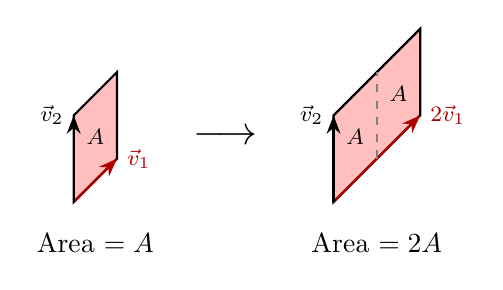
\begin{tikzpicture}[scale=0.55]
  % Original: v1=(1,1), v2=(0,2). Area = 2.
  \begin{scope}
    \fill[red!25] (0,0) -- (1,1) -- (1,3) -- (0,2) -- cycle;
    \draw[thick] (0,0) -- (1,1) -- (1,3) -- (0,2) -- cycle;
    \draw[-{Stealth}, thick, red!70!black] (0,0) -- (1,1)
      node[right, font=\footnotesize]{$\vec{v}_1$};
    \draw[-{Stealth}, thick] (0,0) -- (0,2)
      node[left, font=\footnotesize]{$\vec{v}_2$};
    \node at (0.5, 1.5) {\footnotesize $A$};
    \node[below] at (0.5, -0.5) {Area $= A$};
  \end{scope}

  \node[font=\Large] at (3.5, 1.5) {$\longrightarrow$};

  % Scaled: 2v1=(2,2), v2=(0,2). Area = 4.
  \begin{scope}[shift={(6,0)}]
    \fill[red!25] (0,0) -- (2,2) -- (2,4) -- (0,2) -- cycle;
    \draw[thick] (0,0) -- (2,2) -- (2,4) -- (0,2) -- cycle;
    \draw[-{Stealth}, thick, red!70!black] (0,0) -- (2,2)
      node[right, font=\footnotesize]{$2\vec{v}_1$};
    \draw[-{Stealth}, thick] (0,0) -- (0,2)
      node[left, font=\footnotesize]{$\vec{v}_2$};
    % Split showing two copies
    \draw[dashed, thick, gray] (1,1) -- (1,3);
    \node at (0.5, 1.5) {\footnotesize $A$};
    \node at (1.5, 2.5) {\footnotesize $A$};
    \node[below] at (1, -0.5) {Area $= 2A$};
  \end{scope}
\end{tikzpicture}
\end{center}

$$
\det \begin{pmatrix} k\vec{v}_1 & \vec{v}_2 \end{pmatrix}
= k \cdot \det \begin{pmatrix} \vec{v}_1 & \vec{v}_2 \end{pmatrix}
$$

\vfill
Together, additivity $+$ scaling $=$ \x{multilinearity}.

\end{frame}


% ── Frame 9: Same columns → zero ─────────────────────────
% ADR: Degenerate parallelogram = flat line. The visual is immediate.
\begin{frame}{Property 2: Same Columns $\implies$ Zero Area}

If both sides point in the \x{same direction}, the parallelogram collapses to a \x{line}:

\begin{center}
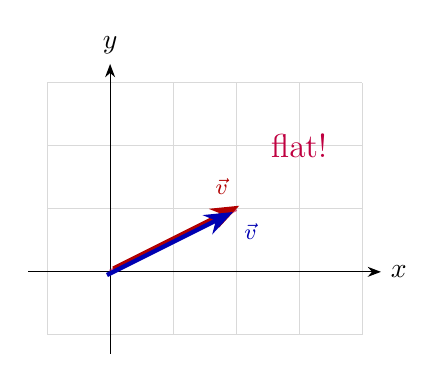
\begin{tikzpicture}[scale=0.8]
  \draw[gray!30, step=1] (-1,-1) grid (4,3);
  \draw[-{Stealth}] (-1.3,0) -- (4.3,0) node[right]{$x$};
  \draw[-{Stealth}] (0,-1.3) -- (0,3.3) node[above]{$y$};

  % Degenerate parallelogram = thick line
  \draw[ultra thick, purple, opacity=0.6] (0,0) -- (2,1);
  \draw[-{Stealth}, ultra thick, red!70!black] (0.05, 0.05) -- (2.05, 1.05)
    node[above left]{\footnotesize $\vec{v}$};
  \draw[-{Stealth}, ultra thick, blue!70!black] (-0.05, -0.05) -- (1.95, 0.95)
    node[below right]{\footnotesize $\vec{v}$};

  \node[purple, font=\large] at (3, 2) {flat!};
\end{tikzpicture}
\end{center}

$$
\det \begin{pmatrix} \vec{v} & \vec{v} \end{pmatrix} = 0
$$

\vfill
A ``parallelogram'' with two identical sides has \x{zero area}.

\end{frame}


% ── Frame 10: Swapping flips sign ─────────────────────────
% ADR: Algebraic consequence derived from Properties 1 & 2.
% No picture needed — the algebra is short and self-contained.
\begin{frame}{Consequence: Swapping Columns Flips the Sign}

Start from Property 2: \quad
$\det \begin{pmatrix} \vec{v}_1{+}\vec{v}_2 & \vec{v}_1{+}\vec{v}_2 \end{pmatrix} = 0$

\vfill
Expand by \x{multilinearity} (Property 1) in both columns:

$$
\underbrace{\det \begin{pmatrix} \vec{v}_1 & \vec{v}_1 \end{pmatrix}}_{=\,0}
+\; \det \begin{pmatrix} \vec{v}_1 & \vec{v}_2 \end{pmatrix}
+\; \det \begin{pmatrix} \vec{v}_2 & \vec{v}_1 \end{pmatrix}
+\; \underbrace{\det \begin{pmatrix} \vec{v}_2 & \vec{v}_2 \end{pmatrix}}_{=\,0}
\;=\; 0
$$

\vfill
Therefore:

$$
\boxed{\;\det \begin{pmatrix} \vec{v}_1 & \vec{v}_2 \end{pmatrix}
= -\det \begin{pmatrix} \vec{v}_2 & \vec{v}_1 \end{pmatrix}\;}
$$

\vfill
\x{Swapping} the two columns \x{flips} the sign of the determinant.

\end{frame}


% ── Frame 11: Normalization ───────────────────────────────
% ADR: The simplest property. Unit square = 1.
\begin{frame}{Property 3: The Unit Square Has Area 1}

The unit square spanned by $\vec{e}_1$ and $\vec{e}_2$ has area $1$:

\begin{center}
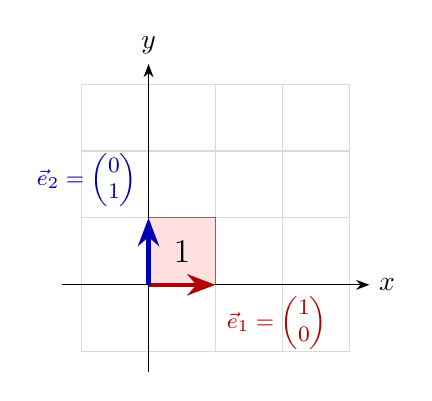
\begin{tikzpicture}[scale=0.85]
  \draw[gray!30, step=1] (-1,-1) grid (3,3);
  \draw[-{Stealth}] (-1.3,0) -- (3.3,0) node[right]{$x$};
  \draw[-{Stealth}] (0,-1.3) -- (0,3.3) node[above]{$y$};

  \filldraw[fill=pink, opacity=0.5] (0,0) -- (1,0) -- (1,1) -- (0,1) -- cycle;

  \draw[-{Stealth}, ultra thick, red!70!black] (0,0) -- (1,0)
    node[below right]{\footnotesize $\vec{e}_1 = \begin{pmatrix} 1 \\ 0 \end{pmatrix}$};
  \draw[-{Stealth}, ultra thick, blue!70!black] (0,0) -- (0,1)
    node[above left]{\footnotesize $\vec{e}_2 = \begin{pmatrix} 0 \\ 1 \end{pmatrix}$};

  \node at (0.5, 0.5) {\large $1$};
\end{tikzpicture}
\end{center}

$$
\det \begin{pmatrix} 1 & 0 \\ 0 & 1 \end{pmatrix} = \det(I_2) = 1
$$

\end{frame}


% ── Frame 12: Definition of determinant ───────────────────
% ADR: Formalize the three properties into a definition. This is the
% transition from "geometric intuition about area" to "mathematical object".
% Students now see that det is DEFINED by the three properties.
\begin{frame}{Definition of Determinant}

\begin{defi}
A function $\det \colon \{\text{square matrices}\} \to \mathbb{R}$ is called a \x{determinant} if it satisfies:

\vspace{0.2cm}
\begin{enumerate}
\item[\textbf{P1.}] \textbf{Multilinearity}: $\det$ is linear in each column separately:
$$
\det(\ldots,\; k\vec{v} + \vec{w},\; \ldots) = k\det(\ldots,\;\vec{v},\;\ldots) + \det(\ldots,\;\vec{w},\;\ldots)
$$
\item[\textbf{P2.}] \textbf{Alternating}: If two columns are equal, $\det = 0$.
\item[\textbf{P3.}] \textbf{Normalization}: $\det(I_n) = 1$.
\end{enumerate}
\end{defi}

\vfill
These three properties \x{axiomatize} the notion of signed volume.

\end{frame}


% ── Frame 13: Two roads to the formula ────────────────────
% ADR: Tension — now that det is defined, can we compute it?
% Signal that there are two independent derivation methods.
\begin{frame}{The $2 \times 2$ Case: Can We Find a Formula?}

For a $2 \times 2$ matrix $\begin{pmatrix} a & b \\ c & d \end{pmatrix}$, what is $\det$?

\vfill

Two independent roads to the answer:

\vfill

\begin{center}
\begin{tabular}{cp{1cm}c}
\textbf{Road 1: Geometric} & & \textbf{Road 2: Algebraic} \\[6pt]
Enclose the parallelogram & & Expand using P1, P2, P3 \\
in a rectangle and subtract & & to derive the formula \\
the remaining pieces & & from the axioms directly
\end{tabular}
\end{center}

\vfill

Both roads must give the \x{same answer} — because the formula is \x{uniquely} determined by P1--P3.

\end{frame}


% ── Frame 14: Rectangle cut-out (Road 1) ─────────────────
% ADR: Figure between question and answer (Macro P10).
% The visual proof: enclose the parallelogram in a rectangle,
% subtract the colored pieces. Students SEE ad-bc emerge.
% Using specific numbers a=2,b=1,c=1,d=2 alongside general labels.
\begin{frame}{Road 1: The Rectangle Cut-Out}

\begin{center}
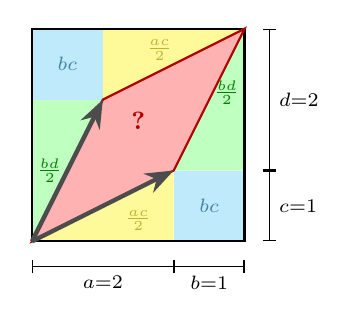
\begin{tikzpicture}[scale=0.9]
  % Fill all regions
  \fill[red!30] (0,0) -- (2,1) -- (3,3) -- (1,2) -- cycle;
  \fill[yellow!40] (0,0) -- (2,0) -- (2,1) -- cycle;
  \fill[yellow!40] (1,2) -- (1,3) -- (3,3) -- cycle;
  \fill[green!25] (0,0) -- (0,2) -- (1,2) -- cycle;
  \fill[green!25] (2,1) -- (3,1) -- (3,3) -- cycle;
  \fill[cyan!25] (2,0) -- (3,0) -- (3,1) -- (2,1) -- cycle;
  \fill[cyan!25] (0,2) -- (1,2) -- (1,3) -- (0,3) -- cycle;

  % Rectangle border
  \draw[thick] (0,0) rectangle (3,3);
  % Parallelogram border
  \draw[red!70!black, thick] (0,0) -- (2,1) -- (3,3) -- (1,2) -- cycle;

  % Vectors
  \draw[-{Stealth}, ultra thick, black!70] (0,0) -- (2,1);
  \draw[-{Stealth}, ultra thick, black!70] (0,0) -- (1,2);

  % Dimension labels
  \draw[|-|] (0,-0.35) -- node[below, font=\scriptsize]{$a{=}2$} (2,-0.35);
  \draw[|-|] (2,-0.35) -- node[below, font=\scriptsize]{$b{=}1$} (3,-0.35);
  \draw[|-|] (3.35,0) -- node[right, font=\scriptsize]{$c{=}1$} (3.35,1);
  \draw[|-|] (3.35,1) -- node[right, font=\scriptsize]{$d{=}2$} (3.35,3);

  % Area labels inside pieces
  \node[red!70!black, font=\small] at (1.5, 1.7) {\textbf{?}};
  \node[yellow!70!black, font=\scriptsize] at (1.5, 0.3) {$\frac{ac}{2}$};
  \node[yellow!70!black, font=\scriptsize] at (1.8, 2.7) {$\frac{ac}{2}$};
  \node[green!50!black, font=\scriptsize] at (0.25, 1.0) {$\frac{bd}{2}$};
  \node[green!50!black, font=\scriptsize] at (2.75, 2.1) {$\frac{bd}{2}$};
  \node[cyan!60!black, font=\scriptsize] at (2.5, 0.5) {$bc$};
  \node[cyan!60!black, font=\scriptsize] at (0.5, 2.5) {$bc$};
\end{tikzpicture}
\end{center}

$$
\underbrace{(a{+}b)(c{+}d)}_{\text{rectangle}}
\;-\; {\color{yellow!70!black}ac}
\;-\; {\color{green!50!black}bd}
\;-\; {\color{cyan!60!black}2bc}
\;=\; \text{\rd{?}}
$$

\end{frame}


% ── Frame 15: Road 1 result ───────────────────────────────
% ADR: Reveal the formula from the geometric method.
\begin{frame}{Road 1: The Formula from Geometry}

Expand the rectangle cut-out:
\begin{align*}
&(a{+}b)(c{+}d) - ac - bd - 2bc \\
={} & ac + ad + bc + bd - ac - bd - 2bc \\
={} & \x{$ad - bc$}
\end{align*}

\vfill

\begin{prop}
$$
\det \begin{pmatrix} a & b \\ c & d \end{pmatrix} = ad - bc
$$
\end{prop}

\end{frame}


% ── Frame 16: Road 2 setup ───────────────────────────────
% ADR: Algebraic derivation from axioms. Step 1: decompose columns
% into standard basis vectors, then expand by multilinearity.
\begin{frame}{Road 2: Deriving from the Axioms}

Write each column in terms of $\vec{e}_1, \vec{e}_2$:
$$
\vec{v}_1 = \begin{pmatrix} a \\ c \end{pmatrix} = a\vec{e}_1 + c\vec{e}_2, \qquad
\vec{v}_2 = \begin{pmatrix} b \\ d \end{pmatrix} = b\vec{e}_1 + d\vec{e}_2
$$

\vfill
Expand by \x{multilinearity} (P1) in the \x{first} column:
$$
\det\begin{pmatrix} \vec{v}_1 & \vec{v}_2 \end{pmatrix}
= \det\begin{pmatrix} a\vec{e}_1 + c\vec{e}_2 & \vec{v}_2 \end{pmatrix}
$$
$$
= a\cdot\det\begin{pmatrix} \vec{e}_1 & \vec{v}_2 \end{pmatrix}
\;+\; c\cdot\det\begin{pmatrix} \vec{e}_2 & \vec{v}_2 \end{pmatrix}
$$

\end{frame}


% ── Frame 17: Road 2 conclusion ──────────────────────────
% ADR: Expand second column, then apply P2 (same=0) and P3 (det I=1).
% Use \underbrace to label each term with the property that kills/evaluates it.
\begin{frame}{Road 2: Applying P2 and P3}

Now expand the \x{second} column in each term:

$$
= ab\underbrace{\det\begin{pmatrix} \vec{e}_1 & \vec{e}_1 \end{pmatrix}}_{\x{$=\,0$}\text{ (P2)}}
+\; ad\underbrace{\det\begin{pmatrix} \vec{e}_1 & \vec{e}_2 \end{pmatrix}}_{\x{$=\,1$}\text{ (P3)}}
$$
$$
+\; cb\underbrace{\det\begin{pmatrix} \vec{e}_2 & \vec{e}_1 \end{pmatrix}}_{\x{$=\,-1$}\text{ (swap)}}
+\; cd\underbrace{\det\begin{pmatrix} \vec{e}_2 & \vec{e}_2 \end{pmatrix}}_{\x{$=\,0$}\text{ (P2)}}
$$

\vfill
Therefore:
$$
\det\begin{pmatrix} a & b \\ c & d \end{pmatrix}
= 0 + ad\cdot 1 + cb\cdot(-1) + 0 = \x{$ad - bc$} \qquad \checkmark
$$

\vfill
Both roads arrive at the \x{same formula} — as they must.

\end{frame}


% ── Frame 18: Solve the warm-up ───────────────────────────
% ADR: Return to the opening question — narrative closure (Macro P8).
\begin{frame}{Solving the Warm-Up}

\begin{columns}[T]
\begin{column}{0.4\textwidth}
\begin{center}
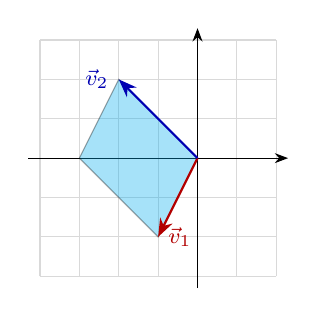
\begin{tikzpicture}[scale=0.5]
  \draw[gray!30, step=1] (-4,-3) grid (2,3);
  \draw[-{Stealth}] (-4.3,0) -- (2.3,0);
  \draw[-{Stealth}] (0,-3.3) -- (0,3.3);
  \filldraw[fill=cyan, opacity=0.35] (0,0) -- (-1,-2) -- (-3,0) -- (-2,2) -- cycle;
  \draw[-{Stealth}, thick, red!70!black] (0,0) -- (-1,-2)
    node[right, font=\footnotesize]{$\vec{v}_1$};
  \draw[-{Stealth}, thick, blue!70!black] (0,0) -- (-2,2)
    node[left, font=\footnotesize]{$\vec{v}_2$};
\end{tikzpicture}
\end{center}
\end{column}
\begin{column}{0.55\textwidth}
$$
\det \begin{pmatrix} -1 & -2 \\ -2 & 2 \end{pmatrix}
$$
$$
= (-1)(2) - (-2)(-2)
$$
$$
= -2 - 4 = \x{-6}
$$

\vspace{0.3cm}
Area $= |-6| = \x{6}$

\vspace{0.3cm}
{\footnotesize The negative sign: $\vec{v}_2$ is \x{clockwise} from $\vec{v}_1$.}
\end{column}
\end{columns}

\end{frame}


% ── Frame 16: Exercises ───────────────────────────────────
\begin{frame}{Practice}

Using the formula $\det \begin{pmatrix} a & b \\ c & d \end{pmatrix} = ad - bc$, calculate:

\vfill

\begin{enumerate}
\item $\det \begin{pmatrix} 1 & 2 \\ 0 & 1 \end{pmatrix} = $

\vfill

\item $\det \begin{pmatrix} 2 & 1 \\ 3 & 2 \end{pmatrix} = $

\vfill

\item $\det \begin{pmatrix} 1 & 0 \\ 8 & 0 \end{pmatrix} = $

\vfill

\item What does it mean geometrically when $\det = 0$?
\end{enumerate}

\vfill

\end{frame}


% ════════════════════════════════════════════════════════════
% §2  Common Mistakes
% ════════════════════════════════════════════════════════════
\section{Common Mistakes}

% ── Frame: Multilinearity is per-column ─────────────────────
\begin{frame}{Multilinearity is \x{Per-Column}}

Recall P1 (multilinearity):
$$
\det(\ldots,\; k\vec{v} + \vec{w},\; \ldots) = k\det(\ldots,\;\vec{v},\;\ldots) + \det(\ldots,\;\vec{w},\;\ldots)
$$

\vfill

The key word: \x{one column at a time}, other columns \x{stay fixed}.

\vfill

\begin{center}
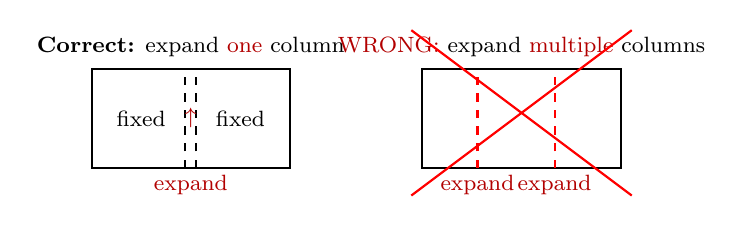
\begin{tikzpicture}[scale=0.7]
  % Good
  \node at (0,2.2) {\footnotesize \textbf{Correct:} expand \rd{one} column};
  \draw[thick] (-1.8,0) rectangle (1.8,1.8);
  \draw[thick,dashed] (-0.1,0) -- (-0.1,1.8);
  \draw[thick,dashed] (0.1,0) -- (0.1,1.8);
  \node at (-0.9,0.9) {\footnotesize fixed};
  \node at (0.9,0.9) {\footnotesize fixed};
  \node[red!70!black] at (0,0.9) {\footnotesize $\uparrow$};
  \node[red!70!black] at (0,-0.3) {\footnotesize expand};

  % Bad
  \node at (6,2.2) {\footnotesize \rd{WRONG:} expand \rd{multiple} columns};
  \draw[thick] (4.2,0) rectangle (7.8,1.8);
  \draw[thick,dashed,red] (5.2,0) -- (5.2,1.8);
  \draw[thick,dashed,red] (6.6,0) -- (6.6,1.8);
  \node[red!70!black] at (5.2,-0.3) {\footnotesize expand};
  \node[red!70!black] at (6.6,-0.3) {\footnotesize expand};
  \draw[red,thick] (4,2.5) -- (8,-0.5);
  \draw[red,thick] (4,-0.5) -- (8,2.5);
\end{tikzpicture}
\end{center}

\end{frame}


% ── Frame: Wrong example ────────────────────────────────────
\begin{frame}{Spot the Error}

\begin{exampleblock}{\rd{WRONG!}}
$$
\det \begin{pmatrix} 1+2 & 1+3 \\ 2+1 & 3+2 \end{pmatrix}
\stackrel{?}{=}
\det \begin{pmatrix} 1 & 1 \\ 2 & 3 \end{pmatrix}
+ \det \begin{pmatrix} 2 & 3 \\ 1 & 2 \end{pmatrix}
$$
\end{exampleblock}

\vfill
\pause

Check: LHS $= \det \begin{pmatrix} 3 & 4 \\ 3 & 5 \end{pmatrix} = 15 - 12 = 3$

\vfill

RHS $= (3-2) + (4-3) = 1 + 1 = 2 \neq 3$

\vfill

The error: expanded \x{both columns simultaneously}.

\end{frame}


% ── Frame: Analogy with multiplication ─────────────────────
\begin{frame}{Why It Fails: The Factor Analogy}

Think of ordinary multiplication:
$$
(\rd{x}+\bl{y})(\rd{a}+\bl{b}) = \rd{xa} + \rd{x}\bl{b} + \bl{y}\rd{a} + \bl{yb}
$$

\vfill

You \x{cannot} skip the cross terms:
$$
(\rd{x}+\bl{y})(\rd{a}+\bl{b}) \;\neq\; \rd{xa} + \bl{yb}
$$

\vfill

Same with $\det$: expanding \x{two} columns at once produces \x{four} terms, not two:

$$
\det\begin{pmatrix} \vec{v}_1 + \vec{w}_1 & \vec{v}_2 + \vec{w}_2 \end{pmatrix}
$$
$$
= \det\begin{pmatrix} \vec{v}_1 & \vec{v}_2 \end{pmatrix}
+ \det\begin{pmatrix} \vec{v}_1 & \vec{w}_2 \end{pmatrix}
+ \det\begin{pmatrix} \vec{w}_1 & \vec{v}_2 \end{pmatrix}
+ \det\begin{pmatrix} \vec{w}_1 & \vec{w}_2 \end{pmatrix}
$$

\end{frame}


% ── Frame: Scaling mistake ─────────────────────────────────
\begin{frame}{Another Trap: $\det(kA) \neq k\det(A)$}

\begin{exampleblock}{\rd{WRONG!}}
$$
\det(2A) \stackrel{?}{=} 2\det(A)
$$
\end{exampleblock}

\vfill
\pause

If $A$ is $3 \times 3$ with columns $\vec{v}_1, \vec{v}_2, \vec{v}_3$, then $2A$ has columns $2\vec{v}_1, 2\vec{v}_2, 2\vec{v}_3$.

$$
\det(2A) = \det(2\vec{v}_1,\; 2\vec{v}_2,\; 2\vec{v}_3)
$$
$$
= 2\det(\vec{v}_1,\; 2\vec{v}_2,\; 2\vec{v}_3)
= 4\det(\vec{v}_1,\; \vec{v}_2,\; 2\vec{v}_3)
= {\color{red!70!black}\boldsymbol{8}}\det(A)
$$

\vfill

\begin{prop}
For an $n \times n$ matrix: $\;\det(kA) = {\color{red!70!black}\boldsymbol{k^n}} \det(A)$
\end{prop}

\end{frame}


% ── Frame: Geometric understanding of k^n ──────────────────
\begin{frame}{Why $k^n$? Think Geometrically}

Scaling every column by $k$ stretches \x{each dimension} by $k$.

\vfill

\begin{center}
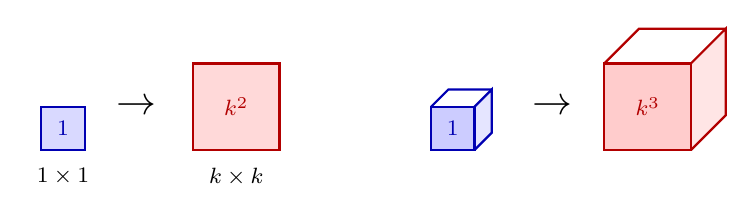
\begin{tikzpicture}[scale=0.55]
  % Original
  \fill[blue!15] (0,0) -- (1,0) -- (1,1) -- (0,1) -- cycle;
  \draw[thick,blue!70!black] (0,0) rectangle (1,1);
  \node[blue!70!black,font=\footnotesize] at (0.5,0.5) {$1$};
  \node[below,font=\footnotesize] at (0.5,-0.2) {$1 \times 1$};

  % 2D scaled
  \begin{scope}[xshift=3.5cm]
  \fill[red!15] (0,0) -- (2,0) -- (2,2) -- (0,2) -- cycle;
  \draw[thick,red!70!black] (0,0) rectangle (2,2);
  \node[red!70!black,font=\footnotesize] at (1,1) {$k^2$};
  \node[below,font=\footnotesize] at (1,-0.2) {$k \times k$};
  \end{scope}

  \node[font=\Large] at (2.2,1) {$\to$};

  % 3D original
  \begin{scope}[xshift=9cm]
  \fill[blue!15] (0,0) -- (1,0) -- (1.4,0.4) -- (0.4,0.4) -- cycle;
  \fill[blue!10] (1,0) -- (1.4,0.4) -- (1.4,1.4) -- (1,1) -- cycle;
  \fill[blue!20] (0,0) -- (1,0) -- (1,1) -- (0,1) -- cycle;
  \draw[thick,blue!70!black] (0,0) -- (1,0) -- (1,1) -- (0,1) -- cycle;
  \draw[thick,blue!70!black] (1,0) -- (1.4,0.4) -- (1.4,1.4) -- (1,1);
  \draw[thick,blue!70!black] (0,1) -- (0.4,1.4) -- (1.4,1.4);
  \node[blue!70!black,font=\footnotesize] at (0.5,0.5) {$1$};
  \end{scope}

  % 3D scaled
  \begin{scope}[xshift=13cm]
  \fill[red!15] (0,0) -- (2,0) -- (2.8,0.8) -- (0.8,0.8) -- cycle;
  \fill[red!10] (2,0) -- (2.8,0.8) -- (2.8,2.8) -- (2,2) -- cycle;
  \fill[red!20] (0,0) -- (2,0) -- (2,2) -- (0,2) -- cycle;
  \draw[thick,red!70!black] (0,0) -- (2,0) -- (2,2) -- (0,2) -- cycle;
  \draw[thick,red!70!black] (2,0) -- (2.8,0.8) -- (2.8,2.8) -- (2,2);
  \draw[thick,red!70!black] (0,2) -- (0.8,2.8) -- (2.8,2.8);
  \node[red!70!black,font=\footnotesize] at (1,1) {$k^3$};
  \end{scope}

  \node[font=\Large] at (11.8,1) {$\to$};
\end{tikzpicture}
\end{center}

\vfill

\begin{itemize}
\item $n=2$: area scales by $k^2$
\item $n=3$: volume scales by $k^3$
\item $n$: ``$n$-volume'' scales by $k^n$
\end{itemize}

\end{frame}


% ── Frame: Practice ─────────────────────────────────────────
\begin{frame}{Practice: True or False?}

Let $A$ be a $4\times 4$ matrix with $\det(A)=3$.

\vfill

\begin{enumerate}
\item $\det(2A) = 2 \cdot 3 = 6$?

\vfill

\item $\det(2A) = 2^4 \cdot 3 = 48$?

\vfill

\item $\det(-A) = -3$?

\vfill

\item $\det(-A) = (-1)^4 \cdot 3 = 3$?
\end{enumerate}

\vfill

\end{frame}


% ════════════════════════════════════════════════════════════
% §3  Column Operations and Switching Matrix
% ════════════════════════════════════════════════════════════
\section{Column Operations and Switching Matrix}

% ── Frame: Column operations preserve det ──────────────────
\begin{frame}{Column Operations Preserve Determinant}

\begin{thm}
Adding a multiple of one column to another does \x{not} change $\det$:
$$
\det(\ldots,\; \vec{v}_i + \lambda\vec{v}_j,\; \ldots,\; \vec{v}_j,\; \ldots)
= \det(\ldots,\; \vec{v}_i,\; \ldots,\; \vec{v}_j,\; \ldots)
$$
\end{thm}

\vfill
\pause

\textbf{Why?} Expand by P1 (multilinearity in column $i$):
$$
\det(\ldots,\; \vec{v}_i + \lambda\vec{v}_j,\; \ldots)
= \det(\ldots,\; \vec{v}_i,\; \ldots)
+ \underbrace{\lambda\det(\ldots,\; \vec{v}_j,\; \ldots,\; \vec{v}_j,\; \ldots)}_{\x{$= 0$} \text{ by P2 (two equal columns)}}
$$

\end{frame}


% ── Frame: Column operations example ───────────────────────
\begin{frame}{Example: Column Operations}

$$
\det\begin{pmatrix} 1 & 3 \\ 2 & 5 \end{pmatrix}
\;\stackrel{c_2 - 3c_1}{=}\;
\det\begin{pmatrix} 1 & 0 \\ 2 & -1 \end{pmatrix}
= -1
$$

\vfill

More generally, for \x{any} number of columns:

$$
\det\begin{pmatrix}
| & | & & | \\
\vec{v}_1 & \vec{v}_2 & \cdots & \vec{v}_n \\
| & | & & |
\end{pmatrix}
$$
$$
=\det\begin{pmatrix}
| & | & & | \\
\vec{v}_1 - \lambda_1\vec{v}_i & \vec{v}_2 - \lambda_2\vec{v}_i & \cdots & \vec{v}_n \\
| & | & & |
\end{pmatrix}
$$
where the $i$-th column is untouched.

\end{frame}


% ── Frame: Linear dependence → det = 0 ────────────────────
\begin{frame}{Dependent Columns $\Rightarrow$ $\det = 0$}

If one column is a linear combination of the others:
$$
\vec{v}_k = \lambda_1\vec{v}_1 + \cdots + \lambda_{k-1}\vec{v}_{k-1} + \lambda_{k+1}\vec{v}_{k+1} + \cdots
$$

\vfill

Subtract those multiples from column $k$:
$$
\det(\ldots,\vec{v}_k,\ldots)
= \det(\ldots,\;\vec{v}_k - \sum_{j\neq k}\lambda_j\vec{v}_j,\;\ldots)
= \det(\ldots,\;\vec{0},\;\ldots)
$$

\vfill

But $\det(\ldots,\vec{0},\ldots) = 0$ (scale by $k{=}0$ in P1).

\vfill

\begin{prop}
If the columns of $A$ are \x{linearly dependent}, then $\det(A)=0$.
\end{prop}

\end{frame}


% ── Frame: Column swapping flips sign ──────────────────────
\begin{frame}{Swapping Two Columns Flips the Sign}

We already saw this for $2\times 2$. In general:

\begin{prop}
Swapping two columns multiplies $\det$ by $-1$.
\end{prop}

\vfill
\pause

\textbf{Proof sketch.} Let $\vec{u},\vec{v}$ be two columns. Consider:
$$
0 = \det(\ldots,\; \vec{u}+\vec{v},\; \ldots,\; \vec{u}+\vec{v},\; \ldots)
$$
Expand by P1 in both positions:
$$
= \det(\ldots,\vec{u},\ldots,\vec{u},\ldots) + \det(\ldots,\vec{u},\ldots,\vec{v},\ldots)
$$
$$
\quad + \det(\ldots,\vec{v},\ldots,\vec{u},\ldots) + \det(\ldots,\vec{v},\ldots,\vec{v},\ldots)
$$

First and last are $0$ (P2). So $\det(\ldots,\vec{u},\ldots,\vec{v},\ldots) = -\det(\ldots,\vec{v},\ldots,\vec{u},\ldots)$.

\end{frame}


% ── Frame: Switching matrix definition ─────────────────────
\begin{frame}{Switching Matrix}

\begin{defi}
A \x{switching matrix} is a matrix where each row and each column has \x{exactly one} nonzero entry, and that entry equals $1$.
\end{defi}

\vfill

Examples:
$$
\begin{pmatrix} 1 & 0 \\ 0 & 1 \end{pmatrix}, \qquad
\begin{pmatrix} 0 & 1 \\ 1 & 0 \end{pmatrix}, \qquad
\begin{pmatrix} 1 & 0 & 0 \\ 0 & 0 & 1 \\ 0 & 1 & 0 \end{pmatrix}, \qquad
\begin{pmatrix} 0 & 0 & 1 & 0 \\ 0 & 0 & 0 & 1 \\ 0 & 1 & 0 & 0 \\ 1 & 0 & 0 & 0 \end{pmatrix}
$$

\vfill

Its $\det$ is either $+1$ or $-1$. But which one?

\end{frame}


% ── Frame: Zigzag method introduction ──────────────────────
\begin{frame}[fragile]{The Zigzag Method}

To find $\det$ of a switching matrix:

\vfill

\begin{enumerate}
\item Draw horizontal and vertical line segments connecting each $1$ to the diagonal entry in its row/column.
\vfill
\item Count the number $m$ of \x{connected loops}.
\vfill
\item $\det = (-1)^{n+m}$
\end{enumerate}

\vfill

\textbf{Why?} Each swap breaks one loop into two. Starting from $I_n$ ($n$ loops, $\det=1$), each swap flips the sign.

\vfill

$n$ loops $\to$ $\det = (-1)^{n+n} = 1 = \det(I_n)$ \checkmark

\end{frame}


% ── Frame: Zigzag example 1 ────────────────────────────────
\begin{frame}[fragile]{Zigzag Example 1}

$$
S_1 = \begin{pmatrix} 0 & 0 & 1 & 0 \\ 0 & 0 & 0 & 1 \\ 0 & 1 & 0 & 0 \\ 1 & 0 & 0 & 0 \end{pmatrix}
$$

\vfill

\begin{center}
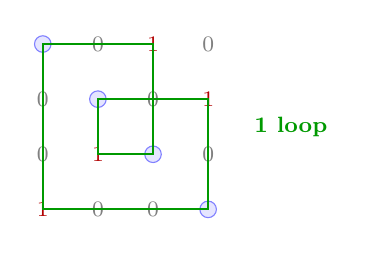
\begin{tikzpicture}[scale=0.7]
  % Grid
  \foreach \i in {1,...,4} {
    \foreach \j in {1,...,4} {
      \node[font=\footnotesize,gray] at (\j,-\i) {$0$};
    }
  }
  % 1s
  \node[font=\footnotesize,red!70!black,fill=white] at (3,-1) {$1$};
  \node[font=\footnotesize,red!70!black,fill=white] at (4,-2) {$1$};
  \node[font=\footnotesize,red!70!black,fill=white] at (2,-3) {$1$};
  \node[font=\footnotesize,red!70!black,fill=white] at (1,-4) {$1$};
  % Diagonal markers
  \foreach \i in {1,...,4} {
    \draw[blue!50,fill=blue!10] (\i,-\i) circle (0.15);
  }
  % Loop: 1→3→2→4→1
  \draw[-{Stealth},thick,green!60!black]
    (1,-1) -- (3,-1) -- (3,-3) -- (2,-3) -- (2,-2) -- (4,-2) -- (4,-4) -- (1,-4) -- cycle;
  \node[green!60!black,font=\footnotesize] at (5.5,-2.5) {\textbf{1 loop}};
\end{tikzpicture}
\end{center}

\vfill

$m = 1$ loop, $n=4$: $\;\det(S_1) = (-1)^{4+1} = \x{-1}$

\end{frame}


% ── Frame: Zigzag example 2 ────────────────────────────────
\begin{frame}[fragile]{Zigzag Example 2}

$$
S_2 = \begin{pmatrix} 0 & 1 & 0 & 0 \\ 1 & 0 & 0 & 0 \\ 0 & 0 & 0 & 1 \\ 0 & 0 & 1 & 0 \end{pmatrix}
$$

\vfill

\begin{center}
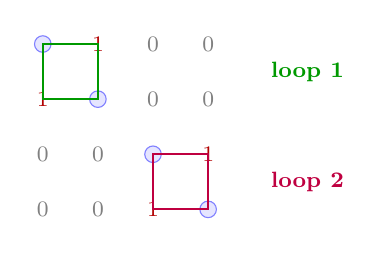
\begin{tikzpicture}[scale=0.7]
  \foreach \i in {1,...,4} {
    \foreach \j in {1,...,4} {
      \node[font=\footnotesize,gray] at (\j,-\i) {$0$};
    }
  }
  \node[font=\footnotesize,red!70!black,fill=white] at (2,-1) {$1$};
  \node[font=\footnotesize,red!70!black,fill=white] at (1,-2) {$1$};
  \node[font=\footnotesize,red!70!black,fill=white] at (4,-3) {$1$};
  \node[font=\footnotesize,red!70!black,fill=white] at (3,-4) {$1$};
  \foreach \i in {1,...,4} {
    \draw[blue!50,fill=blue!10] (\i,-\i) circle (0.15);
  }
  % Loop 1: 1↔2
  \draw[-{Stealth},thick,green!60!black]
    (1,-1) -- (2,-1) -- (2,-2) -- (1,-2) -- cycle;
  % Loop 2: 3↔4
  \draw[-{Stealth},thick,purple]
    (3,-3) -- (4,-3) -- (4,-4) -- (3,-4) -- cycle;
  \node[green!60!black,font=\footnotesize] at (5.8,-1.5) {\textbf{loop 1}};
  \node[purple,font=\footnotesize] at (5.8,-3.5) {\textbf{loop 2}};
\end{tikzpicture}
\end{center}

\vfill

$m = 2$ loops, $n=4$: $\;\det(S_2) = (-1)^{4+2} = \x{+1}$

\end{frame}


% ── Frame: Zigzag practice ─────────────────────────────────
\begin{frame}{Zigzag Practice}

Find the determinant of each switching matrix:

\vfill

\begin{columns}[T]
\begin{column}{0.45\textwidth}
\begin{enumerate}
\item $\begin{pmatrix} 0 & 1 & 0 \\ 0 & 0 & 1 \\ 1 & 0 & 0 \end{pmatrix}$

\vfill

\item $\begin{pmatrix} 0 & 1 & 0 \\ 1 & 0 & 0 \\ 0 & 0 & 1 \end{pmatrix}$
\end{enumerate}
\end{column}
\begin{column}{0.45\textwidth}
\begin{enumerate}
\setcounter{enumi}{2}
\item $\begin{pmatrix} 1 & 0 & 0 & 0 \\ 0 & 0 & 1 & 0 \\ 0 & 0 & 0 & 1 \\ 0 & 1 & 0 & 0 \end{pmatrix}$

\vfill

\item $I_n$ always has $\det = \;$?
\end{enumerate}
\end{column}
\end{columns}

\vfill

\end{frame}


% ════════════════════════════════════════════════════════════
% §4  Cross-Filling Computes Determinant
% ════════════════════════════════════════════════════════════
\section{Cross-Filling Computes Determinant}

% ── Frame: Key insight ─────────────────────────────────────
\begin{frame}{Cross-Filling = Column Operations}

Recall: cross-filling decomposes $A = R_1 + A_1$ where $R_1$ is rank-1 with cross-center $a_1$ and $A_1$ has a \x{zero cross}.

\vfill

\x{Key insight}: this decomposition is just \x{column operations}!

\vfill

\begin{itemize}
\item Subtracting multiples of the pivot column from other columns zeros out the pivot row
\item Column operations \x{preserve} $\det$
\item Then factor out $a_1$ from the pivot column (P1)
\end{itemize}

\vfill

But $A_1$ has a zero at the pivot position --- we cannot cross-fill $A_1$ directly.

\end{frame}


% ── Frame: Annotated remainder definition ─────────────────
\begin{frame}{The Annotated Remainder}

The remainder $A_1$ has a \x{zero cross} --- its pivot position is $0$.

To continue cross-filling, we \x{annotate} that position with a $1$:

\vfill

\begin{defi}
The \x{annotated remainder} $\widehat{A}_1$ is the remainder $A_1$ with the pivot position replaced by $1$.
\end{defi}

\vfill

The annotation \x{remembers} where the previous pivot was --- it marks a ``$1$ has been extracted here.''

\vfill

\begin{thm}
$$
\det(A) = a_1 \cdot \det(\widehat{A}_1)
$$
\end{thm}

\textbf{Why?} Column operations preserve $\det$; factoring $a_1$ from the pivot column gives $\det = a_1 \cdot \det(\widehat{A}_1)$.

\end{frame}


% ── Frame: Iterating ─────────────────────────────────────
\begin{frame}{Iterate: Cross-Fill the Annotated Remainder}

Now cross-fill $\widehat{A}_1$ (it is a full matrix --- ready for the next pivot):
$$
\widehat{A}_1 \;\xrightarrow{\text{cross-fill}}\; \widehat{A}_2 \;\xrightarrow{\text{cross-fill}}\; \cdots \;\xrightarrow{\text{cross-fill}}\; \widehat{A}_n
$$

\vfill

Each step extracts one cross-center $a_i$.

After $n$ steps, every row and column has been used as a pivot exactly once --- the final $\widehat{A}_n$ has $1$'s at all $n$ pivot positions and $0$'s elsewhere.

\vfill

That is exactly a \x{switching matrix} $S = \widehat{A}_n$.

\vfill

\begin{thm}
$$
\boxed{\det(A) = a_1 \cdot a_2 \cdots a_n \cdot \det(S)}
$$
\end{thm}

\end{frame}


% ── Frame: 3×3 example setup ──────────────────────────────
\begin{frame}{Worked Example: Setup}

$$
A = \begin{pmatrix} 2 & 1 & 2 \\ 1 & 3 & 1 \\ 2 & 1 & 3 \end{pmatrix}
$$

\vfill

We compute $\det(A)$ by cross-filling: three steps, three colors.

\vfill

\begin{center}
\rd{Step 1: pivot at $(2,1)$} $\;\to\;$
\bl{Step 2: pivot at $(3,2)$} $\;\to\;$
\gn{Step 3: pivot at $(1,3)$}
\end{center}

\end{frame}


% ── Frame: Step 1 ──────────────────────────────────────────
\begin{frame}{Step 1: Pivot at $(2,1)$, Cross-Center $a_1 = \rd{1}$}

Cross at row 2, column 1. Rank-1 piece = $\frac{1}{a_1}\text{col}_1 \times \text{row}_2$:

$$
\begin{pmatrix}
2 & 1 & 2 \\
\rd{1} & 3 & 1 \\
2 & 1 & 3
\end{pmatrix}
=
\underbrace{\begin{pmatrix}
\rd{2} & \rd{6} & \rd{2} \\
\rd{1} & \rd{3} & \rd{1} \\
\rd{2} & \rd{6} & \rd{2}
\end{pmatrix}}_{R_1\text{ (rank 1)}}
+
\underbrace{\begin{pmatrix}
0 & -5 & 0 \\
0 & 0 & 0 \\
0 & -5 & 1
\end{pmatrix}}_{A_1\text{ (zero cross)}}
$$

\vfill

Annotate: put $1$ at pivot position $(2,1)$:

$$
\det(A) = \rd{1} \cdot \det
\underbrace{\begin{pmatrix} 0 & -5 & 0 \\ \rd{1} & 0 & 0 \\ 0 & -5 & 1 \end{pmatrix}}_{\widehat{A}_1\text{ (annotated remainder)}}
$$

\end{frame}


% ── Frame: Step 2 ──────────────────────────────────────────
\begin{frame}{Step 2: Pivot at $(3,2)$, Cross-Center $a_2 = \bl{-5}$}

Cross-fill the annotated remainder $\widehat{A}_1$:

$$
\begin{pmatrix}
0 & \bl{-5} & 0 \\
\rd{1} & 0 & 0 \\
0 & \bl{-5} & 1
\end{pmatrix}
=
\underbrace{\begin{pmatrix}
0 & \bl{-5} & \bl{1} \\
0 & \bl{0} & \bl{0} \\
0 & \bl{-5} & \bl{1}
\end{pmatrix}}_{R_2}
+
\underbrace{\begin{pmatrix}
0 & 0 & -1 \\
1 & 0 & 0 \\
0 & 0 & 0
\end{pmatrix}}_{A_2}
$$

\vfill

$$
\det(A) = \rd{1}\cdot\bl{(-5)} \cdot \det
\underbrace{\begin{pmatrix} 0 & 0 & -1 \\ \rd{1} & 0 & 0 \\ 0 & \bl{1} & 0 \end{pmatrix}}_{\widehat{A}_2\text{ (annotated)}}
$$

\end{frame}


% ── Frame: Step 3 ──────────────────────────────────────────
\begin{frame}{Step 3: Pivot at $(1,3)$, Cross-Center $a_3 = \gn{-1}$}

Cross-fill $\widehat{A}_2$: pivot at $(1,3)$, cross-center $a_3 = \gn{-1}$.

$$
\widehat{A}_2 = \begin{pmatrix}
0 & 0 & \gn{-1} \\
\rd{1} & 0 & 0 \\
0 & \bl{1} & 0
\end{pmatrix}
=
\underbrace{\begin{pmatrix}
0 & 0 & \gn{-1} \\
0 & 0 & 0 \\
0 & 0 & 0
\end{pmatrix}}_{R_3}
+
\underbrace{\begin{pmatrix}
0 & 0 & 0 \\
1 & 0 & 0 \\
0 & 1 & 0
\end{pmatrix}}_{A_3}
$$

\vfill

Annotate (put $1$ at pivot):
$\;\widehat{A}_3 = \begin{pmatrix} 0 & 0 & \gn{1} \\ \rd{1} & 0 & 0 \\ 0 & \bl{1} & 0 \end{pmatrix} = S$
\quad --- all positions used, this is the \x{switching matrix}!

\end{frame}


% ── Frame: Zigzag for S ───────────────────────────────────
\begin{frame}[fragile]{The Switching Matrix}

$$
S = \begin{pmatrix} 0 & 0 & 1 \\ 1 & 0 & 0 \\ 0 & 1 & 0 \end{pmatrix}
$$

\vfill

\begin{center}
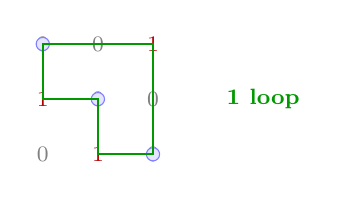
\begin{tikzpicture}[scale=0.7]
  \foreach \i in {1,...,3} {
    \foreach \j in {1,...,3} {
      \node[font=\footnotesize,gray] at (\j,-\i) {$0$};
    }
  }
  \node[font=\footnotesize,red!70!black,fill=white] at (3,-1) {$1$};
  \node[font=\footnotesize,red!70!black,fill=white] at (1,-2) {$1$};
  \node[font=\footnotesize,red!70!black,fill=white] at (2,-3) {$1$};
  \foreach \i in {1,...,3} {
    \draw[blue!50,fill=blue!10] (\i,-\i) circle (0.12);
  }
  \draw[-{Stealth},thick,green!60!black]
    (1,-1) -- (3,-1) -- (3,-3) -- (2,-3) -- (2,-2) -- (1,-2) -- cycle;
  \node[green!60!black,font=\footnotesize] at (5,-2) {\textbf{1 loop}};
\end{tikzpicture}
\end{center}

Cycle $1 \to 3 \to 2 \to 1$: one loop.

$\det(S) = (-1)^{3+1} = \x{+1}$

\end{frame}


% ── Frame: Putting it together ─────────────────────────────
\begin{frame}{Putting It All Together}

$$
\det\begin{pmatrix} 2 & 1 & 2 \\ 1 & 3 & 1 \\ 2 & 1 & 3 \end{pmatrix}
$$

\vfill

$$
= \underbrace{\rd{1}}_{\text{step 1}} \times \underbrace{\bl{(-5)}}_{\text{step 2}} \times \underbrace{\gn{(-1)}}_{\text{step 3}} \times \underbrace{(+1)}_{\text{switching}} = \x{5}
$$

\vfill
\pause

Verify: expand along row 1:
$$
2(9-1) - 1(3-2) + 2(1-6) = 16 - 1 - 10 = 5 \;\checkmark
$$

\end{frame}


% ── Frame: In practice ───────────────────────────────────
\begin{frame}{In Practice: Just Cross-Fill}

The annotated remainder $\widehat{A}$ explains \x{why} the formula works.

But you \x{don't need to write it down}. In practice:

\vfill

\begin{enumerate}
\item Cross-fill as usual (Lecture 8) --- just record each \x{cross-center} $a_i$
\item The pivot positions $(r_1,c_1), (r_2,c_2), \ldots, (r_n,c_n)$ define the switching matrix $S$
\item $\det(A) = a_1 \cdot a_2 \cdots a_n \cdot \det(S)$
\end{enumerate}

\vfill

\begin{alertblock}{When does it fail?}
If at some step \x{no nonzero entry} remains for a pivot $\Rightarrow$ $\det = 0$.
\end{alertblock}

\end{frame}


% ── Frame: Direct example ────────────────────────────────
\begin{frame}{Example: Direct Computation}

$$
A = \begin{pmatrix} 2 & 1 & 3 \\ 1 & 3 & 1 \\ 2 & 1 & 5 \end{pmatrix}
$$

\vfill

Cross-fill (just record pivots):

\vfill

{\renewcommand{\arraystretch}{1.3}
\begin{tabular}{rll}
Step 1: & pivot at $(2,1)$ & cross-center $a_1 = \rd{1}$ \\
Step 2: & pivot at $(1,2)$ & cross-center $a_2 = \bl{-5}$ \\
Step 3: & pivot at $(3,3)$ & cross-center $a_3 = \gn{2}$
\end{tabular}
}

\vfill

Pivot positions: $(2,1), (1,2), (3,3)$ $\Rightarrow$ $S = \left(\begin{smallmatrix} 0 & 1 & 0 \\ 1 & 0 & 0 \\ 0 & 0 & 1 \end{smallmatrix}\right)$, $\;\det(S) = -1$

\vfill

$$
\det(A) = \rd{1} \times \bl{(-5)} \times \gn{2} \times (-1) = \x{10}
$$

\end{frame}


% ── Frame: Exercise ──────────────────────────────────────
\begin{frame}{Exercise}

Compute by cross-filling:

$$
\det\begin{pmatrix} 2 & 3 & 1 \\ 1 & 1 & 2 \\ 3 & 2 & 1 \end{pmatrix}
$$

\vfill

\begin{enumerate}
\item Cross-fill with first pivot at $(2,1)$. Record each cross-center.
\item Read off the switching matrix from the pivot positions.
\item Use zigzag for $\det(S)$.
\item Multiply: $\det = a_1 \cdot a_2 \cdot a_3 \cdot \det(S)$.
\end{enumerate}

\end{frame}


% ── Frame: Exercise solution step 1 ─────────────────────
\begin{frame}{Solution: Step 1}

$$
A = \begin{pmatrix} 2 & 3 & 1 \\ \rd{1} & 1 & 2 \\ 3 & 2 & 1 \end{pmatrix}
$$

Pivot at $(2,1)$, cross-center $a_1 = \rd{1}$.

\vfill

Rank-1 piece: $\frac{1}{1}\begin{pmatrix}2\\1\\3\end{pmatrix}\begin{pmatrix}1&1&2\end{pmatrix} = \begin{pmatrix}\rd{2}&\rd{2}&\rd{4}\\\rd{1}&\rd{1}&\rd{2}\\\rd{3}&\rd{3}&\rd{6}\end{pmatrix}$

\vfill

After subtraction: $\begin{pmatrix}0&1&-3\\0&0&0\\0&-1&-5\end{pmatrix}$ \quad (row 2, col 1 zeroed out)

\end{frame}


% ── Frame: Exercise solution step 2 ─────────────────────
\begin{frame}{Solution: Step 2}

$$
\begin{pmatrix} 0 & 1 & -3 \\ 0 & 0 & 0 \\ 0 & \bl{-1} & -5 \end{pmatrix}
$$

Pivot at $(3,2)$, cross-center $a_2 = \bl{-1}$.

\vfill

Rank-1 piece: $\frac{1}{-1}\begin{pmatrix}1\\0\\-1\end{pmatrix}\begin{pmatrix}0&-1&-5\end{pmatrix} = \begin{pmatrix}0&\bl{1}&\bl{5}\\0&\bl{0}&\bl{0}\\0&\bl{-1}&\bl{-5}\end{pmatrix}$

\vfill

After subtraction: $\begin{pmatrix}0&0&-8\\0&0&0\\0&0&0\end{pmatrix}$ \quad (only entry $(1,3)$ remains)

\end{frame}


% ── Frame: Exercise solution step 3 + result ────────────
\begin{frame}{Solution: Step 3 and Result}

$$
\begin{pmatrix} 0 & 0 & \gn{-8} \\ 0 & 0 & 0 \\ 0 & 0 & 0 \end{pmatrix}
$$

Pivot at $(1,3)$, cross-center $a_3 = \gn{-8}$. Done --- all entries extracted.

\vfill

Pivot positions: $\rd{(2,1)},\; \bl{(3,2)},\; \gn{(1,3)}$ $\;\Rightarrow\;$ switching matrix:

$$
S = \begin{pmatrix} 0 & 0 & \gn{1} \\ \rd{1} & 0 & 0 \\ 0 & \bl{1} & 0 \end{pmatrix}
$$

\vfill

Zigzag: cycle $1 \to 3 \to 2 \to 1$. One loop. $\det(S) = (-1)^{3+1} = +1$.

\vfill

$$
\det(A) = \rd{1} \times \bl{(-1)} \times \gn{(-8)} \times (+1) = \x{8}
$$

\end{frame}


% ── Frame: Exercise 2 ────────────────────────────────────
\begin{frame}{Exercise: $4 \times 4$}

Compute by cross-filling:

$$
\det\begin{pmatrix}
1 & 1 & 0 & 1 \\
1 & 2 & 1 & 0 \\
0 & 1 & 1 & 1 \\
1 & 0 & 1 & 2
\end{pmatrix}
$$

\end{frame}


% ════════════════════════════════════════════════════════════
% §5  Properties of Determinant
% ════════════════════════════════════════════════════════════
\section{Properties of Determinant}

% ── Frame: det(A^T) = det(A) statement ─────────────────────
\begin{frame}{$\det(A^\top) = \det(A)$}

\begin{thm}
For any square matrix $A$: $\;\det(A^\top) = \det(A)$.
\end{thm}

\vfill

This means: everything we said about \x{columns} also holds for \x{rows}.

\vfill

\begin{itemize}
\item Row operations preserve $\det$ (add multiple of one row to another)
\item Two equal rows $\Rightarrow$ $\det = 0$
\item Swapping rows flips sign
\item Dependent rows $\Rightarrow$ $\det = 0$
\end{itemize}

\end{frame}


% ── Frame: det(A^T) proof via cross-filling ────────────────
\begin{frame}{Proof via Cross-Filling}

If $A = R_1 + R_2 + \cdots + R_n$ is a cross-filling for $A$,

then $A^\top = R_1^\top + R_2^\top + \cdots + R_n^\top$ is a cross-filling for $A^\top$.

\vfill
\pause

\textbf{Key observations:}
\begin{enumerate}
\item Transposing a rank-1 cross piece: cross-center \x{stays the same}

(the pivot value doesn't change, just its row/column swap)

\vfill

\item The switching matrix $S^\top$ has the \x{same loops} as $S$

(paths just reverse direction, loop count unchanged)
\end{enumerate}

\vfill

Therefore: $\det(A^\top) = \underbrace{a_1 \cdots a_n}_{\text{same}} \cdot \underbrace{\det(S^\top)}_{\det(S)} = \det(A)$. \qed

\end{frame}


% ── Frame: det(A^T) visual ────────────────────────────────
\begin{frame}[fragile]{Transpose Preserves Loops}

\begin{center}
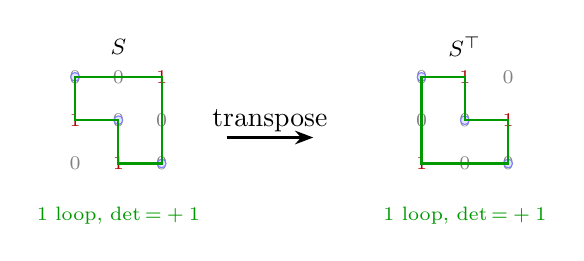
\begin{tikzpicture}[scale=0.55]
  % S: [[0,0,1],[1,0,0],[0,1,0]]
  \node[font=\footnotesize] at (2,-0.3) {$S$};
  \foreach \i in {1,...,3} {
    \foreach \j in {1,...,3} {
      \node[font=\scriptsize,gray] at (\j,-\i) {$0$};
    }
  }
  \node[font=\scriptsize,red!70!black,fill=white] at (3,-1) {$1$};
  \node[font=\scriptsize,red!70!black,fill=white] at (1,-2) {$1$};
  \node[font=\scriptsize,red!70!black,fill=white] at (2,-3) {$1$};
  \foreach \i in {1,...,3} {
    \draw[blue!50,fill=blue!10] (\i,-\i) circle (0.1);
  }
  \draw[-{Stealth},thick,green!60!black]
    (1,-1) -- (3,-1) -- (3,-3) -- (2,-3) -- (2,-2) -- (1,-2) -- cycle;
  \node[green!60!black,font=\scriptsize] at (2,-4.2) {1 loop, $\det{=}+1$};

  % Arrow
  \node[font=\normalsize] at (5.5,-2) {transpose};
  \draw[-{Stealth},thick] (4.5,-2.4) -- (6.5,-2.4);

  % S^T: [[0,1,0],[0,0,1],[1,0,0]]
  \begin{scope}[xshift=8cm]
  \node[font=\footnotesize] at (2,-0.3) {$S^\top$};
  \foreach \i in {1,...,3} {
    \foreach \j in {1,...,3} {
      \node[font=\scriptsize,gray] at (\j,-\i) {$0$};
    }
  }
  \node[font=\scriptsize,red!70!black,fill=white] at (2,-1) {$1$};
  \node[font=\scriptsize,red!70!black,fill=white] at (3,-2) {$1$};
  \node[font=\scriptsize,red!70!black,fill=white] at (1,-3) {$1$};
  \foreach \i in {1,...,3} {
    \draw[blue!50,fill=blue!10] (\i,-\i) circle (0.1);
  }
  \draw[-{Stealth},thick,green!60!black]
    (1,-1) -- (2,-1) -- (2,-2) -- (3,-2) -- (3,-3) -- (1,-3) -- cycle;
  \node[green!60!black,font=\scriptsize] at (2,-4.2) {1 loop, $\det{=}+1$};
  \end{scope}
\end{tikzpicture}
\end{center}

\vfill

$S^\top \neq S$, but the \x{loop count} is the same --- transposing reverses each cycle's direction without splitting or merging loops.

\end{frame}


% ── Frame: What det(A^T) means ─────────────────────────────
\begin{frame}{Why This Matters}

$\det(A^\top) = \det(A)$ gives us a \x{duality}:

\vfill

\begin{center}
\renewcommand{\arraystretch}{1.4}
\begin{tabular}{ccc}
\textbf{Column property} & & \textbf{Row property} \\
\hline
column operations preserve $\det$ & $\leftrightarrow$ & row operations preserve $\det$ \\
equal columns $\Rightarrow$ $\det=0$ & $\leftrightarrow$ & equal rows $\Rightarrow$ $\det=0$ \\
swap columns flips sign & $\leftrightarrow$ & swap rows flips sign \\
dependent columns $\Rightarrow 0$ & $\leftrightarrow$ & dependent rows $\Rightarrow 0$
\end{tabular}
\end{center}

\vfill

From now on, we can freely use \x{either} row or column operations when computing determinants.

\end{frame}


% ── Frame: Block diagonal determinant ─────────────────────
\begin{frame}{Block Diagonal Matrices}

\begin{thm}
If $A$ is block diagonal with square blocks:
$$
\det\begin{pmatrix} B_1 & 0 & \cdots & 0 \\ 0 & B_2 & \cdots & 0 \\ \vdots & \vdots & \ddots & \vdots \\ 0 & 0 & \cdots & B_k \end{pmatrix}
= \det(B_1)\cdot\det(B_2)\cdots\det(B_k)
$$
\end{thm}

\vfill

\textbf{Why?} Cross-filling gives a clean proof.

\end{frame}


% ── Frame: Block diagonal proof ──────────────────────────
\begin{frame}{Proof via Cross-Filling}

When you cross-fill a block diagonal matrix:

\vfill

\begin{itemize}
\item Pick a pivot \x{inside block $B_1$}. The cross (row and column) stays inside $B_1$ --- the zero blocks guarantee that cross-filling doesn't touch other blocks.

\vfill

\item After finishing all pivots in $B_1$, move to $B_2$, then $B_3$, etc.

\vfill

\item Cross-centers: first the pivots of $B_1$, then $B_2$, \ldots

\vfill

\item Switching matrix: block diagonal too --- loops stay within each block.
\end{itemize}

\vfill

So $\det(A) = \underbrace{(\text{pivots of } B_1) \cdot \det(S_1)}_{\det(B_1)} \cdot \underbrace{(\text{pivots of } B_2) \cdot \det(S_2)}_{\det(B_2)} \cdots$

\end{frame}


% ── Frame: Block diagonal example ────────────────────────
\begin{frame}{Example}

$$
\det\begin{pmatrix}
\rd{2} & \rd{1} & 0 & 0 & 0 \\
\rd{1} & \rd{3} & 0 & 0 & 0 \\
0 & 0 & \bl{1} & \bl{2} & \bl{1} \\
0 & 0 & \bl{0} & \bl{1} & \bl{3} \\
0 & 0 & \bl{2} & \bl{1} & \bl{1}
\end{pmatrix}
$$

\vfill

$$
= \det\begin{pmatrix} \rd{2} & \rd{1} \\ \rd{1} & \rd{3} \end{pmatrix}
\times
\det\begin{pmatrix} \bl{1} & \bl{2} & \bl{1} \\ \bl{0} & \bl{1} & \bl{3} \\ \bl{2} & \bl{1} & \bl{1} \end{pmatrix}
$$

\vfill

$$= \rd{5} \times \bl{?}$$

\vfill

{\footnotesize (Compute the $3\times 3$ block by cross-filling!)}

\end{frame}


% ── Frame: Block triangular ──────────────────────────────
\begin{frame}{Block Triangular Matrices}

The same argument works for block \x{upper} or \x{lower} triangular:

\vfill

\begin{thm}
$$
\det\begin{pmatrix} B_1 & * & \cdots & * \\ 0 & B_2 & \cdots & * \\ \vdots & \vdots & \ddots & \vdots \\ 0 & 0 & \cdots & B_k \end{pmatrix}
= \det(B_1)\cdot\det(B_2)\cdots\det(B_k)
$$
\end{thm}

\vfill

\textbf{Why?} Cross-filling block $B_1$ automatically zeros out the $*$ entries above it (they are in the same rows as $B_1$'s pivots). The off-diagonal blocks get cleared for free.

\vfill

In particular: $\det$ of a triangular matrix = product of diagonal entries.

\end{frame}


% ── Frame: Geometric — area under linear map ─────────────
\begin{frame}[fragile]{Geometric Picture: Linear Maps Scale Area}

\begin{columns}
\column{0.45\textwidth}
\begin{center}
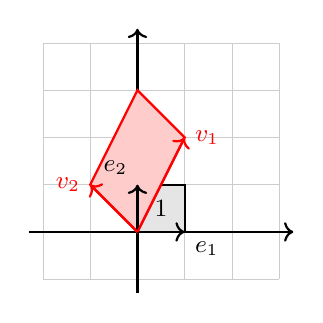
\begin{tikzpicture}[scale=0.6]
% axes
\draw[gray!40, very thin] (-2,-1) grid (3,4);
\draw[thick,->] (-2.3,0) -- (3.3,0);
\draw[thick,->] (0,-1.3) -- (0,4.3);

% unit square
\fill[black!10] (0,0) -- (1,0) -- (1,1) -- (0,1) -- cycle;
\draw[thick] (0,0) -- (1,0) -- (1,1) -- (0,1) -- cycle;
\node at (0.5,0.5) {\small $1$};

% A-parallelogram: A = [[1,-1],[2,1]], cols (1,2) and (-1,1)
\fill[red!20] (0,0) -- (1,2) -- (0,3) -- (-1,1) -- cycle;
\draw[red,thick] (0,0) -- (1,2) -- (0,3) -- (-1,1) -- cycle;

\draw[thick,->] (0,0) -- (1,0) node[below right]{\small $e_1$};
\draw[thick,->] (0,0) -- (0,1) node[above left]{\small $e_2$};
\draw[thick,red,->] (0,0) -- (1,2) node[right]{\small $v_1$};
\draw[thick,red,->] (0,0) -- (-1,1) node[left]{\small $v_2$};
\end{tikzpicture}
\end{center}

\column{0.55\textwidth}

$$A = \begin{pmatrix} 1 & -1 \\ 2 & 1 \end{pmatrix}, \quad \det(A) = \rd{3}$$

\vfill

$A$ maps $e_1 \to v_1,\ e_2 \to v_2$

\vfill

$$\frac{\rd{\text{red parallelogram}}}{\text{unit square}} = |\det(A)| = \rd{3}$$

\vfill

Determinant = \x{area scaling factor}
\end{columns}

\end{frame}


% ── Frame: Geometric — two transformations ────────────────
\begin{frame}[fragile]{Two Transformations: Area Ratios Multiply}

\begin{columns}
\column{0.45\textwidth}
\begin{center}
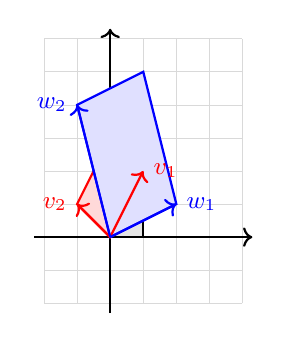
\begin{tikzpicture}[scale=0.42]
% axes
\draw[gray!30, very thin] (-2,-2) grid (4,6);
\draw[thick,->] (-2.3,0) -- (4.3,0);
\draw[thick,->] (0,-2.3) -- (0,6.3);

% unit square
\fill[black!10] (0,0) -- (1,0) -- (1,1) -- (0,1) -- cycle;
\draw[thick] (0,0) -- (1,0) -- (1,1) -- (0,1) -- cycle;

% A-parallelogram: cols (1,2),(-1,1)
\fill[red!15] (0,0) -- (1,2) -- (0,3) -- (-1,1) -- cycle;
\draw[red,thick] (0,0) -- (1,2) -- (0,3) -- (-1,1) -- cycle;

% AB-parallelogram: AB = [[1,-1],[2,1]][[1,1],[-1,2]] = [[2,-1],[1,4]]
% cols (2,1),(-1,4)
\fill[blue!12] (0,0) -- (2,1) -- (1,5) -- (-1,4) -- cycle;
\draw[blue,thick] (0,0) -- (2,1) -- (1,5) -- (-1,4) -- cycle;

\draw[thick,red,->] (0,0) -- (1,2) node[right]{\small $v_1$};
\draw[thick,red,->] (0,0) -- (-1,1) node[left]{\small $v_2$};
\draw[thick,blue,->] (0,0) -- (2,1) node[right]{\small $w_1$};
\draw[thick,blue,->] (0,0) -- (-1,4) node[left]{\small $w_2$};
\end{tikzpicture}
\end{center}

\column{0.55\textwidth}

$$B = \begin{pmatrix} 1 & 1 \\ -1 & 2 \end{pmatrix}, \quad \det(B) = \bl{3}$$

\vfill

$B$ acts \x{on the $A$-grid}: maps $v_i \to w_i$

\vfill

$$\frac{\bl{\text{blue}}}{\rd{\text{red}}} = |\det(B)| = \bl{3}$$

\vfill

$$\frac{\bl{\text{blue}}}{\text{unit}} = \rd{3} \times \bl{3} = 9 = |\det(AB)|$$

\vfill

Area ratios \x{multiply} $\implies \det(AB) = \det(A)\det(B)$
\end{columns}

\end{frame}


% ── Frame: Theorem det(AB) ────────────────────────────────
\begin{frame}{Determinant of a Product}

\begin{thm}
$$\det(AB) = \det(A) \cdot \det(B)$$
\end{thm}

\vfill

\textbf{Geometric intuition:} two successive linear maps scale area by $|\det A|$ then $|\det B|$.

Total scaling = $|\det A| \cdot |\det B| = |\det(AB)|$.

\vfill

\textbf{Now we prove it} using block lower triangular + cross-filling.

\end{frame}


% ── Frame: Cross-filling reveals AB ──────────────────────
\begin{frame}[fragile]{Cross-Filling Reveals the Product}

\textbf{Recall Lecture 10:} Cross-filling $\left(\begin{smallmatrix} A & I \\ I & * \end{smallmatrix}\right)$ with pivots in $A$ $\to$ $*$ is \x{passive} $\to$ reveals $-A^{-1}$.

\vfill

\textbf{Same idea:} form the $2n \times 2n$ block matrix

$$M = \begin{pmatrix} A & 0 \\ I & B \end{pmatrix}$$

\vfill

Cross-fill with pivots from $I$ (bottom-left). The top-right block ($= 0$) is \x{passive} --- it is never read, only written to.

\vfill

Each rank-1 piece from pivot $(n{+}i,\, i) = 1$:

\quad pivot column: $\left(\begin{smallmatrix} a_i \\ e_i \end{smallmatrix}\right)$, \quad pivot row: $(e_i^T,\; b_i^T)$

\quad $\to$ top-right receives $a_i \cdot b_i^T$ (one \x{slice of $AB$})

\vfill

After $n$ steps: sum $= \left(\begin{smallmatrix} A & \rd{AB} \\ I & B \end{smallmatrix}\right)$, \quad remainder $= \left(\begin{smallmatrix} 0 & \rd{-AB} \\ 0 & 0 \end{smallmatrix}\right)$

\end{frame}


% ── Frame: Example setup ─────────────────────────────────
\begin{frame}[fragile]{Example: Cross-Fill $I$ from $M$}

$$A = \begin{pmatrix} 2 & 1 \\ 1 & 2 \end{pmatrix},\quad B = \begin{pmatrix} 2 & 1 \\ 1 & 3 \end{pmatrix}, \quad \det(A)=3,\;\det(B)=5$$

\vfill

$$\underbrace{\begin{pmatrix} 2&1&0&0\\ 1&2&0&0\\ 1&0&2&1\\ 0&1&1&3 \end{pmatrix}}_{M = \left(\begin{smallmatrix} A&0\\ I&B \end{smallmatrix}\right)}
=
\underbrace{\begin{pmatrix} 2&1&\rd{5}&\rd{5}\\ 1&2&\rd{4}&\rd{7}\\ 1&0&2&1\\ 0&1&1&3 \end{pmatrix}}_{\text{sum of 2 rank-1 pieces}}
+
\underbrace{\begin{pmatrix} 0&0&\rd{-5}&\rd{-5}\\ 0&0&\rd{-4}&\rd{-7}\\ 0&0&0&0\\ 0&0&0&0 \end{pmatrix}}_{\text{remainder}}$$

\vfill

Top-right of sum $= \rd{AB} = \left(\begin{smallmatrix}5&5\\4&7\end{smallmatrix}\right)$.
\quad \x{$AB$ appeared!} \quad (Cross-centers: both $= 1$)

\end{frame}


% ── Frame: Example — complete cross-filling ──────────────
\begin{frame}[fragile]{Example: Complete Cross-Filling}

Annotated remainder: $\widehat{A}_2 = \left(\begin{smallmatrix} 0&0&-5&-5\\ 0&0&-4&-7\\ \rd{1}&0&0&0\\ 0&\rd{1}&0&0 \end{smallmatrix}\right)$. \; Continue cross-filling $-AB$:

\vfill

Step 3: pivot $(1,3)$, cross-center $= \bl{-5}$. \quad Step 4: pivot $(2,4)$, cross-center $= \gn{-3}$.

\vfill

Switching matrix $S$: \qquad
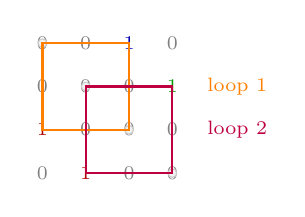
\begin{tikzpicture}[scale=0.55,baseline=(current bounding box.center)]
  \foreach \i in {1,...,4} {
    \foreach \j in {1,...,4} {
      \node[font=\scriptsize,gray] at (\j,-\i) {$0$};
    }
  }
  \node[font=\scriptsize,blue!70!black,fill=white] at (3,-1) {$1$};
  \node[font=\scriptsize,green!60!black,fill=white] at (4,-2) {$1$};
  \node[font=\scriptsize,red!70!black,fill=white] at (1,-3) {$1$};
  \node[font=\scriptsize,red!70!black,fill=white] at (2,-4) {$1$};
  \foreach \i in {1,...,4} {
    \draw[gray!40,fill=gray!10] (\i,-\i) circle (0.1);
  }
  \draw[-{Stealth},thick,orange]
    (1,-1) -- (3,-1) -- (3,-3) -- (1,-3) -- cycle;
  \draw[-{Stealth},thick,purple]
    (2,-2) -- (4,-2) -- (4,-4) -- (2,-4) -- cycle;
  \node[orange,font=\scriptsize] at (5.5,-2) {loop 1};
  \node[purple,font=\scriptsize] at (5.5,-3) {loop 2};
\end{tikzpicture}

\vfill

$$\det(M) = \underbrace{\rd{1}\cdot\rd{1}}_{\text{from }I} \times \underbrace{\bl{(-5)}\cdot\gn{(-3)}}_{\text{from }-AB} \times \underbrace{(-1)^{4+2}}_{2\text{ loops}} = 15$$

$$= \det(A)\det(B) = 3\times 5 = 15 = \det(AB) \;\checkmark$$

\end{frame}


% ── Frame: S_{2n} and T_n definition ─────────────────────
\begin{frame}{The Two Switching Matrices}

Cross-filling $M = \left(\begin{smallmatrix} A & 0 \\ I & B \end{smallmatrix}\right)$ uses pivots from two blocks:

\vfill

\begin{itemize}
\item $I$-block: pivots at $(n{+}i,\; i)$ for $i = 1, \ldots, n$ \quad (cross-centers all $= 1$)
\item $-AB$ block: pivots at $(\sigma(j),\; n{+}j)$ for $j = 1, \ldots, n$
\end{itemize}

\vfill

\begin{defi}
$T_n$ is the $n \times n$ \x{switching matrix} of $-AB$: \; $1$'s at positions $(\sigma(j),\, j)$.

$S_{2n}$ is the full $2n \times 2n$ switching matrix of $M$:
$$
S_{2n} = \begin{pmatrix} 0 & T_n \\ I_n & 0 \end{pmatrix}
$$
\end{defi}

\vfill

In the example: $T_2 = I_2$, \; $S_4 = \left(\begin{smallmatrix} 0&0&1&0 \\ 0&0&0&1 \\ 1&0&0&0 \\ 0&1&0&0 \end{smallmatrix}\right)$.

\end{frame}


% ── Frame: The Key Question ────────────────────────────────
\begin{frame}{The Key Question}

In the example: $S_{4\times 4}$ has \x{2 loops}, and the $2 \times 2$ switching matrix $T_2$ of $-AB$ also has \x{2 loops}.

\vfill

Coincidence?

\vfill

\begin{thm}
For any $\sigma$: \quad loops in $S_{2n}$ $=$ cycles of $\sigma$ $=$ loops in $T_n$.
\end{thm}

\vfill

\textbf{Why this matters:} if true, then $\det(S_{2n}) = (-1)^n \cdot \det(T_n)$, which gives us $\det(AB) = \det(A)\det(B)$.

\vfill

\textbf{Method:} we will \x{deform} each loop of $S_{2n}$ into a loop of $T_n$ by a topological trick --- replacing rectangular detours with shortcuts.

\end{frame}


% ── Frame: Three Diagonals ─────────────────────────────────
\begin{frame}[fragile]{Three Diagonals}

\begin{columns}
\column{0.4\textwidth}
\begin{center}
\begin{tikzpicture}[scale=0.75]
  \draw[gray!40,dashed] (0.5,-2.5) -- (4.5,-2.5);
  \draw[gray!40,dashed] (2.5,-0.5) -- (2.5,-4.5);
  \foreach \i in {1,...,4} {\foreach \j in {1,...,4} {
    \node[font=\tiny,gray!25] at (\j,-\i) {$\cdot$};
  }}
  % Main diagonal
  \foreach \i in {1,...,4} {\fill[gray!40] (\i,-\i) circle (0.12);}
  % Lower diagonal (I)
  \fill[red!70!black] (1,-3) circle (0.12);
  \fill[red!70!black] (2,-4) circle (0.12);
  % Upper diagonal (ghost)
  \draw[orange,dashed,thick] (3,-1) circle (0.16);
  \draw[orange,dashed,thick] (4,-2) circle (0.16);
  % Block labels
  \node[font=\tiny,gray] at (1.5,0) {\textit{diag}};
  \node[font=\tiny,gray] at (3.5,0) {\textit{$-AB$}};
  \node[font=\tiny,gray] at (1.5,-4.8) {\textit{$I$}};
  \node[font=\tiny,gray] at (3.5,-4.8) {\textit{diag}};
\end{tikzpicture}
\end{center}

\column{0.6\textwidth}
The switching matrix has three diagonals:

\vspace{0.5em}

{\small
\renewcommand{\arraystretch}{1.5}
\begin{tabular}{r@{\;:\;}l}
\textbf{main} & $(k,k)$ --- spans two blocks \\
\rd{\textbf{lower}} & $(n{+}i,\;i)$ --- $I$-entries \\
{\color{orange}\textbf{upper}} & $(i,\;n{+}i)$ --- \x{not yet present}
\end{tabular}
}
\end{columns}

\vfill

The upper diagonal will \x{appear} after a topological deformation.

\end{frame}


% ── Frame: The Rectangular Detour ──────────────────────────
\begin{frame}[fragile]{The Rectangular Detour $(\sigma = (1\;2),\; n=2)$}

Trace the zigzag. \x{Between} visits to the upper-right block, the path goes \x{down--left--up}:

\vfill

\begin{columns}
\column{0.5\textwidth}
\begin{center}
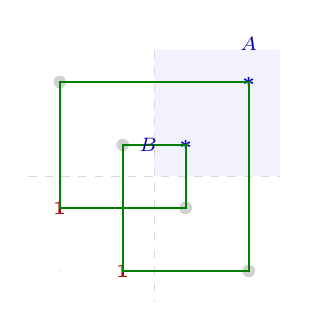
\begin{tikzpicture}[scale=0.8]
  \fill[blue!5] (2.5,-0.5) rectangle (4.5,-2.5);
  \draw[gray!30,dashed] (0.5,-2.5) -- (4.5,-2.5);
  \draw[gray!30,dashed] (2.5,-0.5) -- (2.5,-4.5);
  \foreach \i in {1,...,4} {\foreach \j in {1,...,4} {
    \node[font=\tiny,gray!25] at (\j,-\i) {$\cdot$};
  }}
  \foreach \i in {1,...,4} {\fill[gray!35] (\i,-\i) circle (0.1);}
  \node[font=\scriptsize,red!70!black] at (1,-3) {$\boldsymbol{1}$};
  \node[font=\scriptsize,red!70!black] at (2,-4) {$\boldsymbol{1}$};
  \node[font=\scriptsize,blue!70!black] at (3,-2) {$\boldsymbol{*}$};
  \node[font=\scriptsize,blue!70!black] at (4,-1) {$\boldsymbol{*}$};
  % Full zigzag
  \draw[-{Stealth},thick,green!50!black]
    (1,-1) -- (4,-1) -- (4,-4) -- (2,-4) -- (2,-2) -- (3,-2) -- (3,-3) -- (1,-3) -- cycle;
  % Entry/exit labels
  \node[font=\scriptsize,blue!70!black,above] at (4,-0.65) {$A$};
  \node[font=\scriptsize,blue!70!black,left] at (2.7,-2) {$B$};
\end{tikzpicture}
\end{center}

\column{0.5\textwidth}
The loop visits the upper-right block at $A{=}(1,4)$ and $B{=}(2,3)$.

\vspace{0.8em}

From $A$ to $B$, the zigzag \x{detours} outside:

{\small
$A \xrightarrow{\text{down}} (4,4) \xrightarrow{\text{left}} \rd{(4,2)} \xrightarrow{\text{up}} (2,2) \xrightarrow{\;\;} B$
}

\vspace{0.8em}

Three \x{corners}:
\begin{itemize}
\item $(4,4)$: main diagonal
\item $\rd{(4,2)}$: lower diagonal
\item $(2,2)$: main diagonal
\end{itemize}
\end{columns}

\end{frame}


% ── Frame: The Missing Corner ──────────────────────────────
\begin{frame}[fragile]{The Complete Rectangle}

Draw the full rectangle through the three corners. The 4th corner at {\color{orange}$(2,4)$} sits on the \x{upper diagonal}:

\vfill

\begin{center}
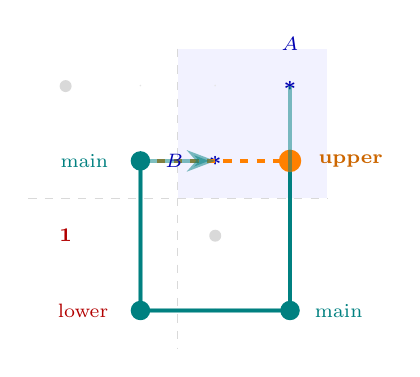
\begin{tikzpicture}[scale=0.95]
  \fill[blue!5] (2.5,-0.5) rectangle (4.5,-2.5);
  \draw[gray!30,dashed] (0.5,-2.5) -- (4.5,-2.5);
  \draw[gray!30,dashed] (2.5,-0.5) -- (2.5,-4.5);
  \foreach \i in {1,...,4} {\foreach \j in {1,...,4} {
    \node[font=\tiny,gray!20] at (\j,-\i) {$\cdot$};
  }}
  \foreach \i in {1,...,4} {\fill[gray!30] (\i,-\i) circle (0.08);}
  \node[font=\scriptsize,red!70!black] at (1,-3) {$\boldsymbol{1}$};
  \node[font=\scriptsize,red!70!black] at (2,-4) {$\boldsymbol{1}$};
  \node[font=\scriptsize,blue!70!black] at (3,-2) {$\boldsymbol{*}$};
  \node[font=\scriptsize,blue!70!black] at (4,-1) {$\boldsymbol{*}$};
  % Rectangle: 3 existing sides (teal, thick)
  \draw[teal,very thick] (4,-2) -- (4,-4);
  \draw[teal,very thick] (4,-4) -- (2,-4);
  \draw[teal,very thick] (2,-4) -- (2,-2);
  % Rectangle: 1 missing side (orange, dashed)
  \draw[orange,very thick,dashed] (2,-2) -- (4,-2);
  % 3 existing corners
  \fill[teal] (4,-4) circle (0.13);
  \node[font=\scriptsize,teal,right] at (4.2,-4) {main};
  \fill[teal] (2,-4) circle (0.13);
  \node[font=\scriptsize,red!70!black,left] at (1.7,-4) {lower};
  \fill[teal] (2,-2) circle (0.13);
  \node[font=\scriptsize,teal,left] at (1.7,-2) {main};
  % Missing corner (orange)
  \fill[orange] (4,-2) circle (0.15);
  \node[font=\scriptsize,orange!80!black,right] at (4.25,-2) {\textbf{upper}};
  % Detour path (over the existing sides)
  \draw[-{Stealth},ultra thick,teal,opacity=0.5]
    (4,-1) -- (4,-4) -- (2,-4) -- (2,-2) -- (3,-2);
  % Entry/exit
  \node[font=\scriptsize,blue!70!black,above] at (4,-0.65) {$A$};
  \node[font=\scriptsize,blue!70!black,left] at (2.7,-2) {$B$};
\end{tikzpicture}
\end{center}

\vfill

{\color{teal}\textbf{Existing}} (3 sides): $A \to (4,4) \to \rd{(4,2)} \to (2,2) \to B$ --- outside the block. \quad
{\color{orange}\textbf{Missing}} (dashed): $(2,2) \to (4,2)$ --- \x{through the upper diagonal}.

\end{frame}


% ── Frame: Topological Deformation ─────────────────────────
\begin{frame}[fragile]{Three Corners $\to$ One Corner}

Replace the {\color{teal}3-side detour} with the {\color{orange}missing side}:

\vfill

\begin{columns}
\column{0.5\textwidth}
\begin{center}
\textbf{Before} {\small (3 corners, outside)}

\vspace{0.3em}

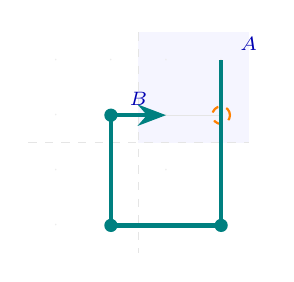
\begin{tikzpicture}[scale=0.7]
  \fill[blue!4] (2.5,-0.5) rectangle (4.5,-2.5);
  \draw[gray!20,dashed] (0.5,-2.5) -- (4.5,-2.5);
  \draw[gray!20,dashed] (2.5,-0.5) -- (2.5,-4.5);
  \foreach \i in {1,...,4} {\foreach \j in {1,...,4} {
    \node[font=\tiny,gray!15] at (\j,-\i) {$\cdot$};
  }}
  % Rectangle outline
  \draw[gray!20,thin] (2,-2) -- (4,-2) -- (4,-4) -- (2,-4) -- cycle;
  % 3 existing corners
  \fill[teal] (4,-4) circle (0.12);
  \fill[teal] (2,-4) circle (0.12);
  \fill[teal] (2,-2) circle (0.12);
  % Missing corner (dashed)
  \draw[orange,dashed,thick] (4,-2) circle (0.16);
  % Detour path (3 sides)
  \draw[-{Stealth},ultra thick,teal]
    (4,-1) -- (4,-4) -- (2,-4) -- (2,-2) -- (3,-2);
  % Labels
  \node[font=\scriptsize,blue!70!black] at (4.5,-0.7) {$A$};
  \node[font=\scriptsize,blue!70!black] at (2.5,-1.7) {$B$};
\end{tikzpicture}
\end{center}

\column{0.5\textwidth}
\begin{center}
\textbf{After} {\small (1 corner, inside)}

\vspace{0.3em}

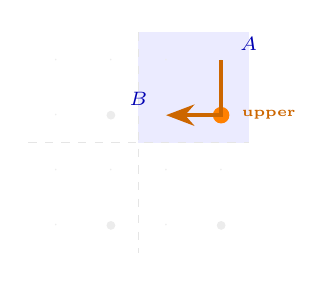
\begin{tikzpicture}[scale=0.7]
  \fill[blue!8] (2.5,-0.5) rectangle (4.5,-2.5);
  \draw[gray!20,dashed] (0.5,-2.5) -- (4.5,-2.5);
  \draw[gray!20,dashed] (2.5,-0.5) -- (2.5,-4.5);
  \foreach \i in {1,...,4} {\foreach \j in {1,...,4} {
    \node[font=\tiny,gray!15] at (\j,-\i) {$\cdot$};
  }}
  % Faded old corners
  \fill[gray!15] (4,-4) circle (0.08);
  \fill[gray!15] (2,-4) circle (0.08);
  \fill[gray!15] (2,-2) circle (0.08);
  % New corner (solid orange)
  \fill[orange] (4,-2) circle (0.15);
  \node[font=\tiny,orange!80!black,right] at (4.2,-2) {\textbf{upper}};
  % Shortcut path (1 side)
  \draw[-{Stealth},ultra thick,orange!80!black]
    (4,-1) -- (4,-2) -- (3,-2);
  % Labels
  \node[font=\scriptsize,blue!70!black] at (4.5,-0.7) {$A$};
  \node[font=\scriptsize,blue!70!black] at (2.5,-1.7) {$B$};
\end{tikzpicture}
\end{center}
\end{columns}

\vfill

\x{Same two endpoints} $A$ and $B$. The loop goes $A \to \cdots \to B \to \cdots \to A$.

We only changed one path ($A$ to $B$) --- the loop \x{does not break}.

\end{frame}


% ── Frame: Step 1 ─────────────────────────────────────────
\begin{frame}[fragile]{Step 1: Replace the First Detour}

Deform the {\color{teal}first rectangle} ($A \to B$):

\vfill

\begin{columns}
\column{0.5\textwidth}
\begin{center}
\textbf{Original zigzag}

\vspace{0.3em}

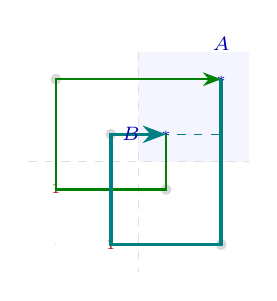
\begin{tikzpicture}[scale=0.7]
  \fill[blue!4] (2.5,-0.5) rectangle (4.5,-2.5);
  \draw[gray!25,dashed] (0.5,-2.5) -- (4.5,-2.5);
  \draw[gray!25,dashed] (2.5,-0.5) -- (2.5,-4.5);
  \foreach \i in {1,...,4} {\foreach \j in {1,...,4} {
    \node[font=\tiny,gray!20] at (\j,-\i) {$\cdot$};
  }}
  \foreach \i in {1,...,4} {\fill[gray!30] (\i,-\i) circle (0.1);}
  \node[font=\tiny,red!70!black] at (1,-3) {$1$};
  \node[font=\tiny,red!70!black] at (2,-4) {$1$};
  \node[font=\tiny,blue!70!black] at (3,-2) {$*$};
  \node[font=\tiny,blue!70!black] at (4,-1) {$*$};
  % Second detour (unchanged, green)
  \draw[-{Stealth},thick,green!50!black]
    (3,-2) -- (3,-3) -- (1,-3) -- (1,-1) -- (4,-1);
  % First detour (being replaced, teal)
  \draw[-{Stealth},very thick,teal]
    (4,-1) -- (4,-4) -- (2,-4) -- (2,-2) -- (3,-2);
  % Rectangle outline
  \draw[teal,thin,dashed] (2,-2) -- (4,-2);
  % Labels
  \node[font=\scriptsize,blue!70!black,above] at (4,-0.65) {$A$};
  \node[font=\scriptsize,blue!70!black,left] at (2.7,-2) {$B$};
\end{tikzpicture}
\end{center}

\column{0.5\textwidth}
\begin{center}
\textbf{After step 1}

\vspace{0.3em}

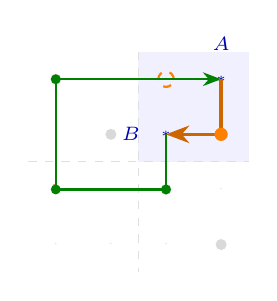
\begin{tikzpicture}[scale=0.7]
  \fill[blue!6] (2.5,-0.5) rectangle (4.5,-2.5);
  \draw[gray!25,dashed] (0.5,-2.5) -- (4.5,-2.5);
  \draw[gray!25,dashed] (2.5,-0.5) -- (2.5,-4.5);
  \foreach \i in {1,...,4} {\foreach \j in {1,...,4} {
    \node[font=\tiny,gray!20] at (\j,-\i) {$\cdot$};
  }}
  \foreach \i in {1,...,4} {\fill[gray!30] (\i,-\i) circle (0.1);}
  \node[font=\tiny,red!70!black] at (1,-3) {$1$};
  \node[font=\tiny,blue!70!black] at (3,-2) {$*$};
  \node[font=\tiny,blue!70!black] at (4,-1) {$*$};
  % Rectangle outline for second detour: 3 existing sides (green)
  \draw[green!50!black,thick] (3,-2) -- (3,-3);
  \draw[green!50!black,thick] (3,-3) -- (1,-3);
  \draw[green!50!black,thick] (1,-3) -- (1,-1);
  % Missing side (green dashed)
  \draw[green!50!black,thick,dashed] (1,-1) -- (3,-1);
  % 3 existing corners
  \fill[green!50!black] (3,-3) circle (0.09);
  \fill[green!50!black] (1,-3) circle (0.09);
  \fill[green!50!black] (1,-1) circle (0.09);
  % Missing corner on upper diagonal
  \draw[orange,dashed,thick] (3,-1) circle (0.14);
  % Second detour path (green, over the rectangle sides)
  \draw[-{Stealth},thick,green!50!black]
    (3,-2) -- (3,-3) -- (1,-3) -- (1,-1) -- (4,-1);
  % First detour REPLACED (orange, inside block)
  \draw[-{Stealth},very thick,orange!80!black]
    (4,-1) -- (4,-2) -- (3,-2);
  % New corner from step 1
  \fill[orange] (4,-2) circle (0.12);
  % Labels
  \node[font=\scriptsize,blue!70!black,above] at (4,-0.65) {$A$};
  \node[font=\scriptsize,blue!70!black,left] at (2.7,-2) {$B$};
\end{tikzpicture}
\end{center}
\end{columns}

\vfill

{\color{teal}Detour 1} replaced by {\color{orange}shortcut}. The {\color{green!50!black}second rectangle} now visible --- {\color{green!50!black}dashed} = next replacement.

\end{frame}


% ── Frame: Step 2 ─────────────────────────────────────────
\begin{frame}[fragile]{Step 2: Replace the Second Detour}

Now deform the {\color{green!50!black}second rectangle} ($B \to A$):

\vfill

\begin{columns}
\column{0.5\textwidth}
\begin{center}
\textbf{After step 1}

\vspace{0.3em}

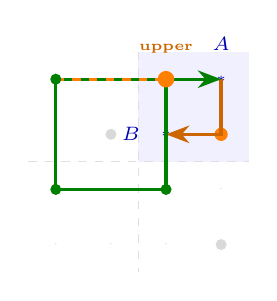
\begin{tikzpicture}[scale=0.7]
  \fill[blue!6] (2.5,-0.5) rectangle (4.5,-2.5);
  \draw[gray!25,dashed] (0.5,-2.5) -- (4.5,-2.5);
  \draw[gray!25,dashed] (2.5,-0.5) -- (2.5,-4.5);
  \foreach \i in {1,...,4} {\foreach \j in {1,...,4} {
    \node[font=\tiny,gray!20] at (\j,-\i) {$\cdot$};
  }}
  \foreach \i in {1,...,4} {\fill[gray!30] (\i,-\i) circle (0.1);}
  \node[font=\tiny,red!70!black] at (1,-3) {$1$};
  \node[font=\tiny,blue!70!black] at (3,-2) {$*$};
  \node[font=\tiny,blue!70!black] at (4,-1) {$*$};
  \fill[orange] (4,-2) circle (0.12);
  % First detour (already replaced, orange)
  \draw[-{Stealth},very thick,orange!80!black]
    (4,-1) -- (4,-2) -- (3,-2);
  % Second detour path (green, drawn first so rectangle shows on top)
  \draw[-{Stealth},very thick,green!50!black]
    (3,-2) -- (3,-3) -- (1,-3) -- (1,-1) -- (4,-1);
  % Rectangle outline ON TOP: 3 existing sides (green solid)
  \draw[green!50!black,very thick] (3,-1) -- (3,-3);
  \draw[green!50!black,very thick] (3,-3) -- (1,-3);
  \draw[green!50!black,very thick] (1,-3) -- (1,-1);
  % Missing side ON TOP (orange dashed, clearly visible)
  \draw[orange,very thick,dashed] (1,-1) -- (3,-1);
  % 3 existing corners
  \fill[green!50!black] (3,-3) circle (0.1);
  \fill[green!50!black] (1,-3) circle (0.1);
  \fill[green!50!black] (1,-1) circle (0.1);
  % Missing corner on upper diagonal
  \fill[orange] (3,-1) circle (0.15);
  \node[font=\tiny,orange!80!black,above] at (3,-0.7) {\textbf{upper}};
  % Labels
  \node[font=\scriptsize,blue!70!black,above] at (4,-0.65) {$A$};
  \node[font=\scriptsize,blue!70!black,left] at (2.7,-2) {$B$};
\end{tikzpicture}
\end{center}

\column{0.5\textwidth}
\begin{center}
\textbf{After step 2}: loop in block

\vspace{0.3em}

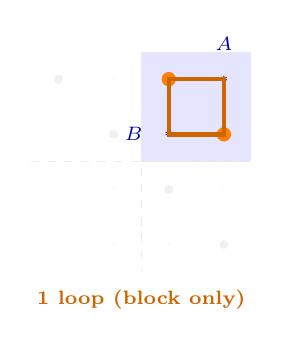
\begin{tikzpicture}[scale=0.7]
  \fill[blue!10] (2.5,-0.5) rectangle (4.5,-2.5);
  \draw[gray!15,dashed] (0.5,-2.5) -- (4.5,-2.5);
  \draw[gray!15,dashed] (2.5,-0.5) -- (2.5,-4.5);
  \foreach \i in {1,...,4} {\foreach \j in {1,...,4} {
    \node[font=\tiny,gray!10] at (\j,-\i) {$\cdot$};
  }}
  \foreach \i in {1,...,4} {\fill[gray!12] (\i,-\i) circle (0.08);}
  \node[font=\tiny,blue!70!black] at (3,-2) {$*$};
  \node[font=\tiny,blue!70!black] at (4,-1) {$*$};
  % Both corners on upper diagonal
  \fill[orange] (3,-1) circle (0.13);
  \fill[orange] (4,-2) circle (0.13);
  % Deformed loop (entirely in block)
  \draw[-{Stealth},ultra thick,orange!80!black]
    (4,-1) -- (4,-2) -- (3,-2) -- (3,-1) -- cycle;
  \node[orange!80!black,font=\scriptsize] at (2.5,-5) {\textbf{1 loop (block only)}};
  % Labels
  \node[font=\scriptsize,blue!70!black,above] at (4,-0.65) {$A$};
  \node[font=\scriptsize,blue!70!black,left] at (2.7,-2) {$B$};
\end{tikzpicture}
\end{center}
\end{columns}

\vfill

Both detours replaced. The loop now \x{lives entirely in the upper-right block}.

Corners alternate: \bl{$-AB$ entries} and {\color{orange}upper diagonal} $=$ a \x{$T_n$ zigzag}!

\end{frame}


% ── Frame: Diagonal Pivots ────────────────────────────────
\begin{frame}[fragile]{Degenerate Case $(\sigma = \text{id},\; n=2)$}

\bl{$-AB$ entries} at $(1,3)$ and $(2,4)$ --- \x{already on the upper diagonal}:

\vfill

\begin{columns}
\column{0.5\textwidth}
\begin{center}
\textbf{Before}: $S_{4\times 4}$

\vspace{0.5em}

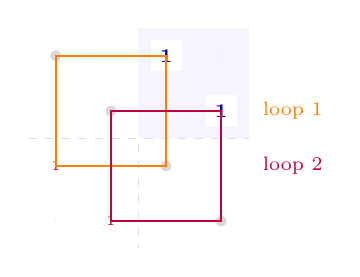
\begin{tikzpicture}[scale=0.7]
  \draw[gray!25,dashed] (0.5,-2.5) -- (4.5,-2.5);
  \draw[gray!25,dashed] (2.5,-0.5) -- (2.5,-4.5);
  \fill[blue!4] (2.5,-0.5) rectangle (4.5,-2.5);
  \foreach \i in {1,...,4} {\foreach \j in {1,...,4} {
    \node[font=\tiny,gray!20] at (\j,-\i) {$\cdot$};
  }}
  \foreach \i in {1,...,4} {\fill[gray!30] (\i,-\i) circle (0.1);}
  \node[font=\tiny,red!70!black] at (1,-3) {$1$};
  \node[font=\tiny,red!70!black] at (2,-4) {$1$};
  \node[font=\scriptsize,blue!70!black,fill=white] at (3,-1) {$\boldsymbol{1}$};
  \node[font=\scriptsize,blue!70!black,fill=white] at (4,-2) {$\boldsymbol{1}$};
  \draw[-{Stealth},thick,orange]
    (1,-1) -- (3,-1) -- (3,-3) -- (1,-3) -- cycle;
  \draw[-{Stealth},thick,purple]
    (2,-2) -- (4,-2) -- (4,-4) -- (2,-4) -- cycle;
  \node[orange,font=\scriptsize] at (5.3,-2) {loop 1};
  \node[purple,font=\scriptsize] at (5.3,-3) {loop 2};
\end{tikzpicture}
\end{center}

\column{0.5\textwidth}
\begin{center}
\textbf{After}: upper-right block

\vspace{0.5em}

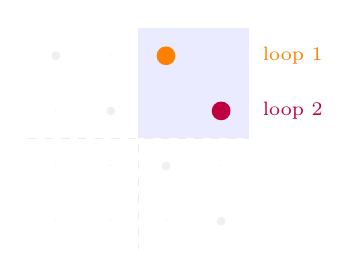
\begin{tikzpicture}[scale=0.7]
  \draw[gray!15,dashed] (0.5,-2.5) -- (4.5,-2.5);
  \draw[gray!15,dashed] (2.5,-0.5) -- (2.5,-4.5);
  \fill[blue!8] (2.5,-0.5) rectangle (4.5,-2.5);
  \foreach \i in {1,...,4} {\foreach \j in {1,...,4} {
    \node[font=\tiny,gray!10] at (\j,-\i) {$\cdot$};
  }}
  \foreach \i in {1,...,4} {\fill[gray!12] (\i,-\i) circle (0.08);}
  \fill[orange] (3,-1) circle (0.17);
  \fill[purple] (4,-2) circle (0.17);
  \node[orange,font=\scriptsize] at (5.3,-1) {loop 1};
  \node[purple,font=\scriptsize] at (5.3,-2) {loop 2};
\end{tikzpicture}
\end{center}
\end{columns}

\vfill

Each rectangle is \x{degenerate}: the missing 4th corner \x{coincides} with the $-AB$ entry itself.

Each loop collapses to a single point on the upper diagonal $\to$ \x{2 separate loops}.

\end{frame}


% ── Frame: The Reduction ──────────────────────────────────
\begin{frame}{The Reduction}

\begin{center}
\renewcommand{\arraystretch}{1.5}
\begin{tabular}{c|c|c}
 & $\sigma$ cycles & $S_{2n}$ loops \\ \hline
$n{=}2$, $\sigma=\text{id}$ & 2 & 2 \\
$n{=}2$, $\sigma=(1\;2)$ & 1 & 1 \\ \hline
$n{=}3$, $\sigma=(1\;2\;3)$ & 1 & 1 \\
$n{=}3$, $\sigma=(1\;2)(3)$ & 2 & 2 \\
\end{tabular}
\end{center}

\vfill

\begin{thm}
Loops in $S_{2n}$ $=$ cycles of $\sigma$ $=$ loops in $T_n$
\end{thm}

\vfill

\textbf{Why?} Each rectangular detour through the diagonal $+$ $I$ blocks can be deformed into a shortcut through the \x{upper diagonal}. This reduces the $2n \times 2n$ zigzag to an $n \times n$ zigzag in the upper-right block --- same loops, smaller matrix.

\end{frame}


% ── Frame: Sign Comparison ───────────────────────────────
\begin{frame}{Sign Comparison}

Both $S_{2n}$ and $T_n$ have the same number of loops $p$.

\vfill

$$\det(S_{2n}) = (-1)^{2n+p} \qquad \det(T_n) = (-1)^{n+p}$$

\vfill

$$\frac{\det(S_{2n})}{\det(T_n)} = (-1)^{(2n+p)-(n+p)} = (-1)^n$$

\vfill

$$\boxed{\det(S_{2n}) = (-1)^n \cdot \det(T_n)}$$

\vfill

The deformation from $2n$ to $n$ positions contributes exactly $(-1)^n$ to the sign --- always.

\end{frame}



% ── Frame: General proof ─────────────────────────────────
\begin{frame}{Proof (General)}

$M = \begin{pmatrix} A & 0 \\ I & B \end{pmatrix}$, \; $\det(M) = \det(A)\det(B)$ \; (block lower triangular).

\vfill

Cross-fill $M$: $n$ pivots from $I$ (all $= 1$), then $n$ pivots from $-AB$.

$$\det(M) = \underbrace{1^n}_{\text{from } I} \times \text{(pivots of }{-AB}\text{)}  \times \det(S_{2n})$$

The $I$-entries form $n$ linked pairs $\to$ same loops as $T_n$:
$\;\det(S_{2n}) = (-1)^n \cdot \det(T_n)$

\vfill

$$\det(M) = \underbrace{(-1)^n \cdot \det(-AB)}_{\text{pivots}\times\det(S)} = (-1)^n \cdot (-1)^n \det(AB) = \det(AB)$$

\vfill

\begin{center}
\fbox{$\det(A)\det(B) = \det(M) = \det(AB)$} \quad $\square$
\end{center}

\end{frame}


% ── Frame: Corollary — invertibility ─────────────────────
\begin{frame}{Corollary: Invertibility and Determinant}

\begin{prop}
$A$ is invertible $\iff$ $\det(A) \neq 0$
\end{prop}

\vfill

($\Rightarrow$) \; If $A$ is invertible:
$$\det(A)\cdot\det(A^{-1}) = \det(AA^{-1}) = \det(I_n) = 1$$
so $\det(A) \neq 0$.

\vfill

($\Leftarrow$) \; If $\det(A) \neq 0$: cross-filling gives $n$ \x{nonzero} pivots $\to$ rank $n$ $\to$ invertible.

\end{frame}


% ── Frame: More corollaries ──────────────────────────────
\begin{frame}{More Consequences}

\begin{enumerate}
\item If $A$ is invertible:
$$\det(A^{-1}) = \frac{1}{\det(A)}$$

\vfill

\item For any positive integer $k$:
$$\det(A^k) = \det(A)^k$$

\vfill

\item Recall from \S2:
$$\det(\lambda A) = \lambda^n \det(A)$$
\end{enumerate}

\end{frame}


\end{document}
